%% 
%% Copyright 2007-2020 Elsevier Ltd
%% 
%% This file is part of the 'Elsarticle Bundle'.
%% ---------------------------------------------
%% 
%% It may be distributed under the conditions of the LaTeX Project Public
%% License, either version 1.2 of this license or (at your option) any
%% later version.  The latest version of this license is in
%%    http://www.latex-project.org/lppl.txt
%% and version 1.2 or later is part of all distributions of LaTeX
%% version 1999/12/01 or later.
%% 
%% The list of all files belonging to the 'Elsarticle Bundle' is
%% given in the file `manifest.txt'.
%% 
%% Template article for Elsevier's document class `elsarticle'
%% with harvard style bibliographic references

\documentclass[preprint,12pt,authoryear]{elsarticle}

%% Use the option review to obtain double line spacing
%% \documentclass[authoryear,preprint,review,12pt]{elsarticle}

%% Use the options 1p,twocolumn; 3p; 3p,twocolumn; 5p; or 5p,twocolumn
%% for a journal layout:
%% \documentclass[final,1p,times,authoryear]{elsarticle}
%% \documentclass[final,1p,times,twocolumn,authoryear]{elsarticle}
%% \documentclass[final,3p,times,authoryear]{elsarticle}
%% \documentclass[final,3p,times,twocolumn,authoryear]{elsarticle}
%% \documentclass[final,5p,times,authoryear]{elsarticle}
%% \documentclass[final,5p,times,twocolumn,authoryear]{elsarticle}

%% For including figures, graphicx.sty has been loaded in
%% elsarticle.cls. If you prefer to use the old commands
%% please give \usepackage{epsfig}

%% The amssymb package provides various useful mathematical symbols
\usepackage{amssymb}
%% The amsthm package provides extended theorem environments
%% \usepackage{amsthm}

%% The lineno packages adds line numbers. Start line numbering with
%% \begin{linenumbers}, end it with \end{linenumbers}. Or switch it on
%% for the whole article with \linenumbers.
%% \usepackage{lineno}

\usepackage{multirow}
\usepackage{hyperref}
\usepackage{graphics}
\usepackage{booktabs}
\usepackage{multirow}
\usepackage{caption}
\usepackage{amsmath}
\usepackage{siunitx}

\journal{Journal of Hydrology}

\begin{document}

\begin{frontmatter}

%% Title, authors and addresses

%% use the tnoteref command within \title for footnotes;
%% use the tnotetext command for theassociated footnote;
%% use the fnref command within \author or \affiliation for footnotes;
%% use the fntext command for theassociated footnote;
%% use the corref command within \author for corresponding author footnotes;
%% use the cortext command for theassociated footnote;
%% use the ead command for the email address,
%% and the form \ead[url] for the home page:
%% \title{Title\tnoteref{label1}}
%% \tnotetext[label1]{}
%% \author{Name\corref{cor1}\fnref{label2}}
%% \ead{email address}
%% \ead[url]{home page}
%% \fntext[label2]{}
%% \cortext[cor1]{}
%% \affiliation{organization={},
%%            addressline={}, 
%%            city={},
%%            postcode={}, 
%%            state={},
%%            country={}}
%% \fntext[label3]{}

\title{Optimizing warnings from hydrologic ensemble prediction systems for improved decision making}

%% use optional labels to link authors explicitly to addresses:
%% \author[label1,label2]{}
%% \affiliation[label1]{organization={},
%%             addressline={},
%%             city={},
%%             postcode={},
%%             state={},
%%             country={}}
%%
%% \affiliation[label2]{organization={},
%%             addressline={},
%%             city={},
%%             postcode={},
%%             state={},
%%             country={}}

\author[inst1]{Jesús Casado-Rodríguez}
\author[inst1]{Peter Salamon}
\author[inst2]{Stefania Grimaldi}
\author[inst2]{Corentin Carton De Wiart}
\author[inst2]{Christel Prudhomme}
\author[inst2]{Calum Baugh}
\author[inst2]{Ervin Zsoter}
\author[inst3]{Ilias Pechlivanidis}
\author[inst3]{Nina Bosshard}
\author[inst4]{Michaela Mikulickova}

\affiliation[inst1]{organization={European Commission, Joint Research Centre, Directorate E - Space, Security and Migration},%Department and Organization
            addressline={Via Enrico Fermi 2749}, 
            city={Ispra},
            postcode={21027}, 
            state={(VA)},
            country={Italy}}

\affiliation[inst2]{organization={European Centre for Medium Range Weather Forecasts},%Department and Organization
            addressline={Shinfield Park}, 
            city={Reading},
            postcode={WC2R 2LS}, 
            country={UK}}

\affiliation[inst3]{organization={Swedish Meteorological and Hydrological Institute},%Department and Organization
            city={Norrköping},
            country={Sweden}}

\affiliation[inst4]{organization={Slovak Hydrometeorological Institute},%Department and Organization
            city={Bratislava},
            country={Slovakia}}

\begin{abstract}
Early Warning Systems are critical in mitigating the impact of floods, the most frequent and economically damaging natural hazard worldwide. These systems rely on hydrological simulations driven by meteorological forecasts, both of which are inherently uncertain. Ensemble Prediction Systems (EPS) were developed decades ago to account for these uncertainties by generating multiple future scenarios that portray the forecast uncertainty. The advantages of probabilistic modelling have been proven over the last decades both in the fields of meteorology and hydrology. In order to issue a flood warning, the probabilities provided by EPS need to be converted into dichotomous values of "warning" or "not warning". This conversion is often done by application of thresholds, whose definition is pivotal for the final skill of the system. While meteorological and hydrological models are under continuous development —higher spatial and temporal resolution, better process representation, improved calibrations—, the methodologies for converting discharge forecasts into flood warnings lack continuous evaluation.
In this paper, we use discharge simulations from the European Flood Awareness System (EFAS) to assess the skill of the four NWP models of different nature —probabilistic and deterministic—within the system, and search for methods to combine the different NWP into a grand ensemble that enhances the overall skill. Additionally, we evaluate the effects of the current notification criteria —probability threshold and persistence— and determine their optimal values. Our results demonstrate that probabilistic NWP models outperform deterministic ones, which demonstrate skill only at short lead times. Additionally, our findings suggest that the persistence criterion is beneficial for removing inconsistencies between consecutive forecasts in deterministic NWP, but should be omitted from probabilistic systems. By applying optimal notification criteria to a single probabilistic NWP, we observe an improvement of up to 6.4\% in skill compared with the current EFAS procedure, which employs four NWP models.  When compared with the best probabilistic NWP, grand ensembles only yield significant improvements in skill (up to 4.2\%) within the first two days lead time, when the individual assessment of deterministic NWP showed skill. Two methods to create the grand ensemble stand out from the rest —equiprobability among all model runs or skill weighted—; we discuss benefits and drawbacks of these two approaches. Overall, our study underscores the importance of selecting appropriate flood notification criteria and limits the added value of deterministic NWP in a grand ensemble to the shortest lead time range.
\end{abstract}

%%Graphical abstract
%\begin{graphicalabstract}
%
\includegraphics{grabs}
%\end{graphicalabstract}

%%Research highlights
\begin{highlights}
\item Research highlight 1
\item Research highlight 2
\end{highlights}

\begin{keyword}
%% keywords here, in the form: keyword \sep keyword
EFAS \sep flood warnings \sep floods early warning system \sep probabilistic forecasting
%% PACS codes here, in the form: \PACS code \sep code
\PACS 0000 \sep 1111
%% MSC codes here, in the form: \MSC code \sep code
%% or \MSC[2008] code \sep code (2000 is the default)
\MSC 0000 \sep 1111
\end{keyword}

\end{frontmatter}

%% \linenumbers

\section{Introduction}
\label{sec:introduction}

Floods are the natural disaster that causes the biggest economical losses in Europe \cite{WMO2021}. In the European Union (EU), flood damages amounted to a total cost of approximately 280 billion EUR in the period 1980-2022, representing 43\% of all meteorological hazards \cite{EEA2023}. The historical data show an increasing tendency in flood damages over Europe \cite{EEA2023, Paprotny2018}, and climate projections indicate an exacerbation of this trend with increasing frequency and severity of extreme events \cite{Alfieri2017, IPCC2023}. In this scenario, Flood Early Warning Systems (FEWS) emerge as one of the multiple adaptation measures to be taken. The major flood event in the Elbe River in 2002 triggered the development of the European Flood Awareness system (EFAS), a continental scale FEWS that has been running since 2005 and whose monetary value has been proven \cite{Pappenberger2015b}. The magnitude of the flood that hit Germany and Belgium in July 2021, the most costly in the last 40 years, was a reminder of the importance of FEWS and their continuous improvement. On a global scale, the United Nations launched the initiative Early Warnings for All to ensure that the entire World population is warned about weather, water and climate hazards by 2027 \cite{UN2023}. Continental systems like EFAS, and more importantly its global counterpart GloFAS (Global Flood Awareness System), are cornerstones for achieving the goals of this UN initiative.

FEWS rely on meteorological forecasts generated by Numerical Weather Prediction (NWP) models. Over the past thirty years, Ensemble Prediction Systems (EPS) have been develop within the realm of NWP models to account for uncertainties in the initial conditions. EPS offer equiprobable forecasts at any given time and location, enabling the quantification and dissemination of probabilistic forecasts. Compared to deterministic models, EPS have proven increased consistency across consecutive forecasts \cite{Buizza2008} and improved precipitation forecasts at longer lead times \cite{Molteni1996}.

Approximately two decades ago, the success of EPS in meteorology led to the adoption of this paradigm in flood forecasting \cite{Diomede2008, Bartholmes2009, Thielen2009a, Yang2020}. Hydrological Ensemble Predictions Systems (HEPS) propagate the uncertainties in the meteorological forecasts by forcing hydrological models with all the individual members of the ensemble. Although this approach is the most common, it only considers the uncertainty in the initial meteorological condition, but does not include other sources of uncertainty, such as model representation or model parameterization \cite{Cloke2009}. 

The decision to issue weather-related warnings, such as floods, is delicate as it might result in significant costs, either due to unpreparedness if an event is missed or the mobilization of resources in false alarms. Weather forecasting systems often issue a higher number of false alarms than missed events \cite{Bouttier2023}, despite the potential risk of eroding trust in the system, known as the 'cry wolf' effect \cite{LeClerc2015}. Their research showed that an increase in false alarms diminishes the credibility of the system, leading end-users to disregard precautionary measures. However, they also demonstrated that incorporating uncertainty estimates in warning messages can assist users in making informed decisions. Therefore, HEPS have the potential to enhance both the skill and trustworthiness of flood warning system, with particular attention to the balance between false alarms and missed events.

The European Flood Awareness System (EFAS) is the hydrological forecast component of the Copernicus Emergency Management Services (CEMS) of the European Commission \cite{Thielen2009a}. EFAS is an operational system that monitors and forecasts floods in a extensive European domain, encompassing not only European Union member states. Its primary objective is to enable proactive measures in anticipation of significant flood events. EFAS functions as a complementary system to national or regional counterparts, with a specific focus on trans-boundary rivers and medium-range forecasts. 

Since 2020, EFAS has been generating forecasts twice a day, with a 6-hour resolution and lead times extending up to 10 days. It couples four weather forecasts of diverse nature, both deterministic and probabilistic, with the distributed, physically-based hydrological model LISFLOOD-OS \cite{Burek2013a}. The simulation produces a set of water fluxes and state variables, from which river discharge is utilized to issue flood warnings, also referred to as notifications. EFAS employs a threshold exceedance approach for issuing warnings \cite{Bartholmes2009}, where continuous discharge time series are converted into binary series of exceedance or not-exceedance over a discharge threshold (the 5-year return period). In their work, Bartholmes et al. \cite{Bartholmes2009} developed a notification criteria based on two types of persistence: persistence in a particular forecast is determined by the number of NWP members predicting the exceedance, while persistence over several forecast establishes the reliability of the flood signal only if a number of consecutive forecasts predict the flood. We will use the term "probability of exceedance" to refer to the first type of persistence.  The number of NWP members exceeding the discharge threshold can be translated into a probability, assuming equiprobability among the members of a particular NWP. On the other hand, we will use the term "persistence" to denote only to the consistency among consecutive forecasts. 

The criteria applied in EFAS have evolved and currently stand at a 30\% probability threshold and a persistence of 3 consecutive forecasts. These criteria are independently applied to the two deterministic and the two probabilistic NWP models, issuing a notification only if at least one of the models of each type predicts the flood. Additionally, EFAS notifications are exclusively dispatched to locations with a minimum catchment area of 2000 km² and for lead times longer than 48 hours. The first limit is based on the inferior hydrological performance in smaller catchments, while the second limit is a consequence of EFAS serving as a supplementary system to national or regional services.

Previous studies have examined the skill of EFAS notifications \cite{Bartholmes2009} and the response of end users \cite{Demeritt2013}. However, the continuous advances in NWP performance \cite{Bauer2015}, as well as in the resolution and representation of hydrological processes in EFAS \cite{EFASv4.0, EFASv5.0}, requires a new evaluation of the notification criteria to harness the potential of the system. The objective of this analysis is to assess the skill of a continental flood forecasting system like EFAS in its current state, and explore new notification criteria that can maximize its  skill. 

In particular, the first goal is to determine the value of combining several NWP models of different natures in a single system, specifically seeking the appropriate combination method to create a grand ensemble from the individual NWP models. The second goal is to optimize the two notification criteria (probability threshold and persistence), analysing the interplay between them and reconsidering whether the persistence criterion is meaningful in a purely probabilistic approach. The third and final goal is to analyse the evolution of the notification skill with catchment area to discern if the newer, higher resolution models are skillful in smaller catchments.

To address our research questions, we conducted an analysis of  EFAS4 discharge simulations for the period 2020-2023. Section \ref{sec:data} enumerates the datasets used in the analysis. Section \ref{sec:methods} explains the two experiments that analyse the skill of individual NWP models and different combinations of those models, the criteria optimization process, and the skill metrics we targeted. Section \ref{sec:results} follows a similar structure, presenting first the skill of individual NWP, then that of several combination methods, and ends with an exploration of the relationship between notification skill and catchment area. Section \ref{sec:discussion} discusses the importance of the spatio-temporal framework and target metric in such skill analysis, the trade-offs between the notification criteria, the benefits of combining NWP models, and the challenges in selecting a combination method.

\section{Data}
\label{sec:data}

The data used in this analysis is taken from the operational setup of the European Flood Awareness  System (EFAS) in its version 4 \cite{EFASv4.0}. EFAS generates a hydrological forecast twice a day (00 and 12 UTC) forced by the meteorological forecast of 4 different numerical weather prediction (NWP) models, whose characteristics are specified in Table \ref{tab:NWP_chars}. EFAS combines probabilistic models (COS and ENS) and deterministic models (DWD and HRES) to produce flood warnings.

\begin{table}
    \centering
    \caption{Characteristics of the numerical weather prediction models used in EFAS4.}
    \footnotesize %\small
    \begin{tabular}{llllll} 
        \toprule
        Model & Provider & Acronym & \parbox{2cm}{Max.\\ lead time} & \parbox{2cm}{No.\\ ensembles} & \parbox{2cm}{Spatial \\ resolution} \\
        \midrule
        COSMO-LEPS & & COS & 5.5 days & 20 & $\sim$ 7 km \\
        ICON-EU/ICON & DWD & DWD & 7 days & 1 & $\sim$ 6.5-13 km \\
        HRES & ECMWF & HRES & 10 days & 1 & $\sim$ 9 km \\ 
        ENS & ECMWF & ENS & 10 days &  51 & $\sim$ 18 km \\ 
        \bottomrule
    \end{tabular}
    \label{tab:NWP_chars}
\end{table}

The study period spans from the release of EFAS4 in October 2020 until June 2023. For this period we will use the EFAS forecasts as the discharge prediction and the EFAS reanalysis as a proxy of discharge observations. Using reanalysis as ground truth avoids the limitation of observational data (e.g. gaps in the observed time series, difference in recorded period...), and reduces model representation and calibration errors from the analysis. The previous data sets must be converted from a continuous variable (discharge) into binary events of exceedance or not exceedance over a threshold. Following the current EFAS setup, the flood threshold is the discharge associated with the 5 year return period, which was computed from the simulated discharge the EFAS4 long run (1991-2023)  by fitting a Gumbel distribution to the annual maxima.

Spatial resolution of EFAS!!

Unlike the original EFAS skill assessment \cite{Bartholmes2009}, the analysis will not focus on all the river cells in the model, which might cause an autocorrelation problem, but only at real gauging stations. From the almost 4000 gauging stations in the EFAS database, a selection was made based on two conditions: the contributing area must be larger than 500 km², and the hydrological performance in terms of modified KGE (Kling-Gupta efficiency) \cite{Gupta2009, Knoben2019} must not be lower than 0.50. We set a lower bound on the catchment area because the relatively coarse spatial resolution of NWP and the length of the EFAS time step (6 h) limit EFAS performance in small catchments. The condition based on hydrological performance ensures that the assumption of using model simulations as proxies for observations is valid. In the end, 1979 gauging stations were included in the analysis, which account for a total of 1683 events (exceedances over the 5 year threshold) during the study period. As it will be explained in section \ref{sec:methods_OPT}, the optimization of the notification criteria will be done on the subset of 1239 stations whose contributing area is larger than 2000 km²; the total amount of events in this subset is 874.

\section{Methods}
\label{sec:methods}

The skill assessment comprises four steps, as depicted schematically in Figure \ref{fig:scheme}: (a) transformation of both observed and forecasted discharge time series into corresponding time series of the probability of exceeding the 5-year return period; (b) construction of an exceedance probability matrix that consolidates the overlapping forecasts, followed by identification of predicted events through the application of specific notification criteria on that matrix; (c) calculation of the contingency table (hits, misses and false alarms), (d) evaluation of the skill of the system across all possible combinations of the notification criteria.

\begin{figure}
    \centering
    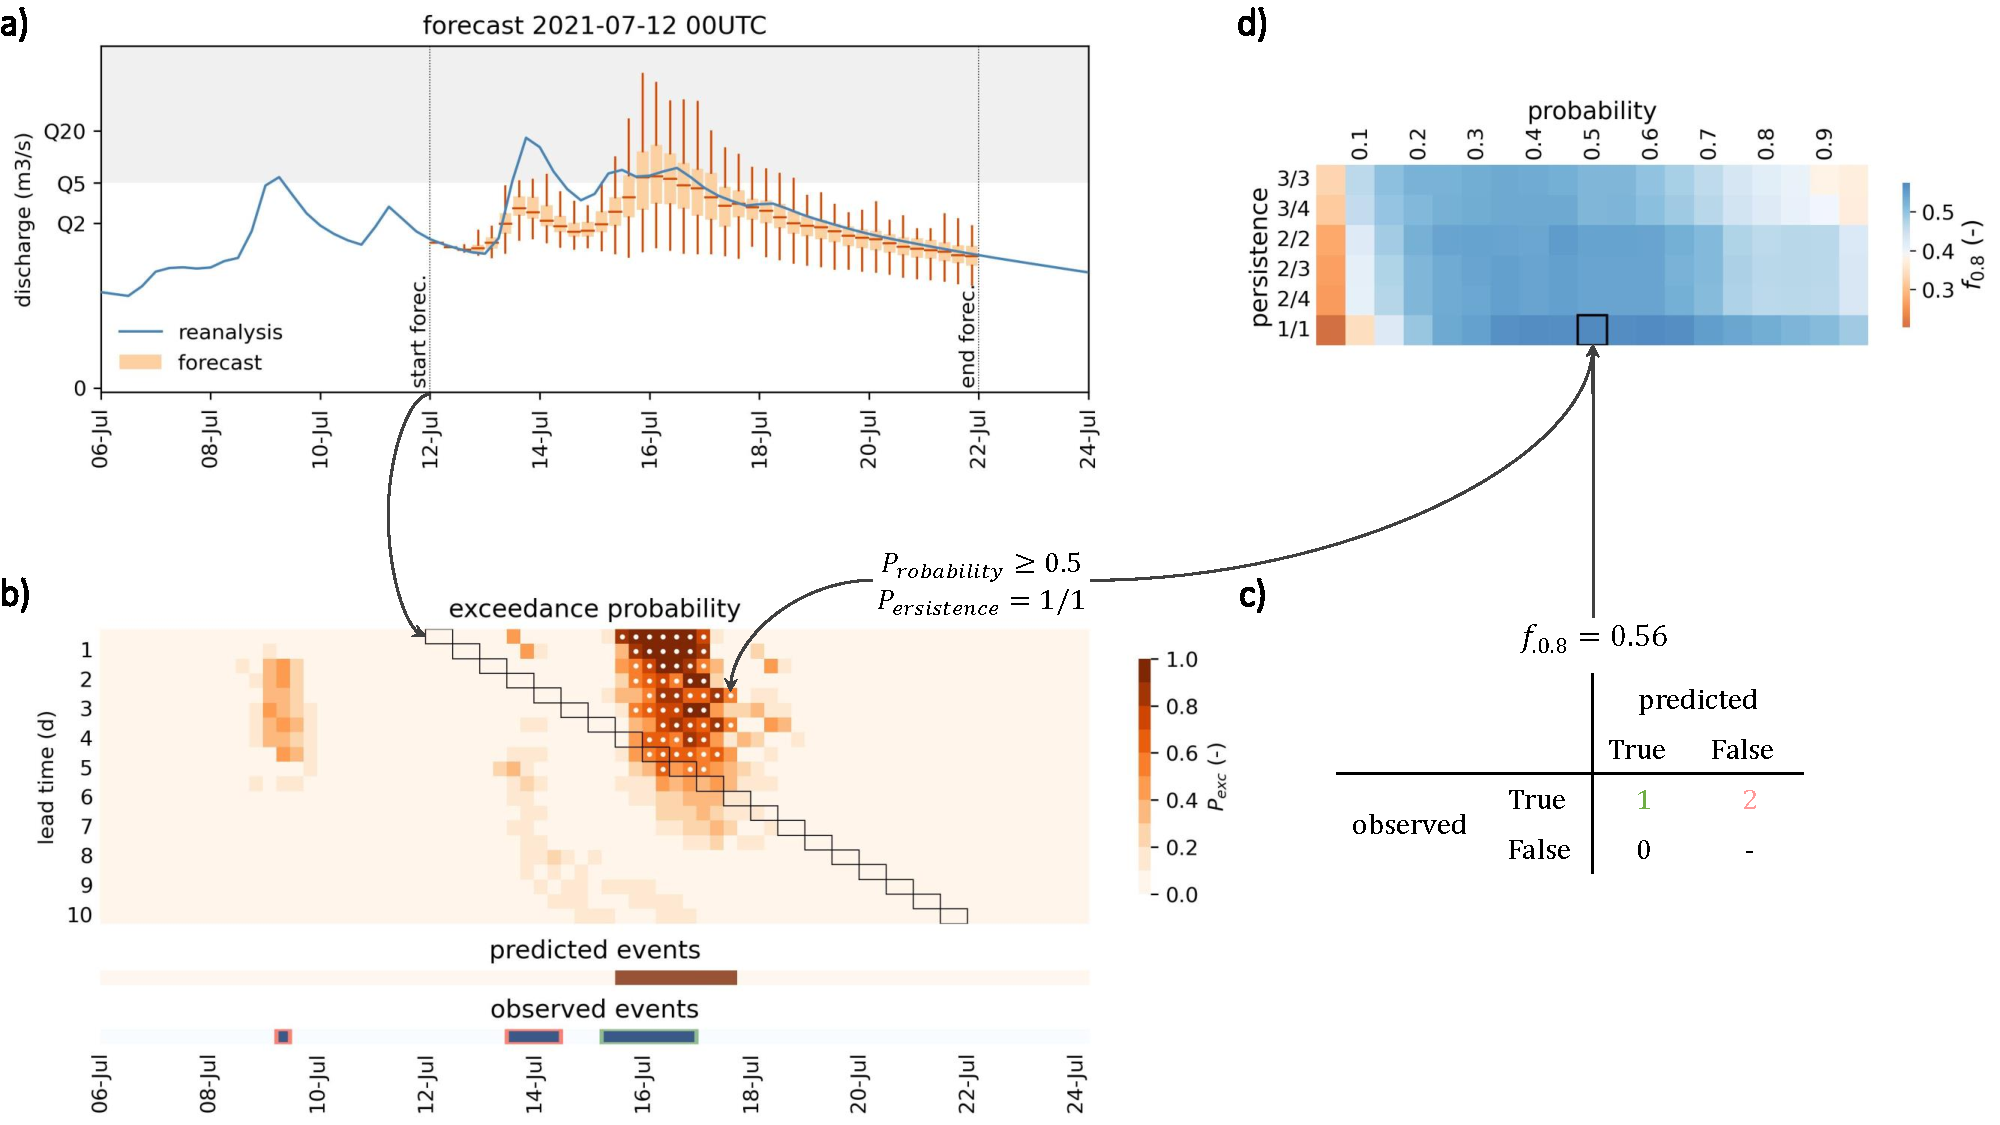
\includegraphics[width=1\linewidth]{figures/study_layout.pdf}
    \caption{Overview of the skill assessment framework. a) Hydrographs comparing observed and forecasted discharge with the discharge associated to the 5-year return period. b) Matrix of total exceedance probability (white dots signify pairs of date and lead time that meet the notification criteria, whereas black rectangles delineate the conversion of the forecast hydrograph from panel (a) into the probability matrix) and identification of predicted events for specific values of the probability threshold and persistence. c) Confusion matrix for the selected station, constructed based on the applied notification criteria . d) Evaluation of the f-score across all combinations of probability threshold and persistence; the black square highlights the skill score corresponding to the notification criteria in panel (b).}
    \label{fig:scheme}
\end{figure}

\subsection{Exceedance over threshold}
\label{sec:methods_exceedance}

The notification process starts by converting the continuous time series of the target variable into time series of exceedance or non-exceedance over a predefined threshold. Within EFAS, flood notifications are based on discharge, and the critical threshold is the discharge associated with a 5-year return period ($Q_5$) generated from a 30-year historical simulation. While alternative alert systems might rely on disparate variables, such as precipitation \cite{Bouttier2023} or river stage \cite{Nevo2022}, and employ different thresholds for defining events, the underlying methodology remains similar. 

The application of the discharge threshold yields distinct outcomes when comparing a singular time series—like observations or deterministic forecasts—with an ensemble forecast. In the former case, the time series is converted into a binary sequence, where 0 represents non-exceedance and 1 denotes exceedance. Conversely, ensemble forecasts lead to a probability time series, with values fluctuating between 0 and 1. Since forecasts —both deterministic and probabilistic— are generated more frequently (every 12 hours) than the forecast horizon, they overlap. To address this, the ensemble forecasts are restructured into an exceedance probability matrix that connects each time step to increasing lead times, as illustrated in panel (b) of Figure \ref{fig:scheme}. Such a configuration simplifies both the analysis and the subsequent computations. Within this matrix, an individual forecast is represented by a diagonal (black rectangles). The uppermost rows of the matrix are associated with forecasts nearer to the actual event, where the probability of accurate prediction generally increases. For instance, in the example in Figure \ref{fig:scheme}, the flood event occurring around July 16 was predicted with a 50\% probability five days in advance, increasing close to certainty within two days of the event.

\subsubsection{Combination of NWP}
\label{sec:methods_COMB}

One of the particularities of EFAS is the simultaneous use of 4 NWP, both deterministic and probabilistic. Other warning systems may use only 1 NWP, whether it is deterministic or probabilistic. The purpose of using multiple NWP is to leverage the strengths of each model. Thus, a primary aim of this study is to develop an effective method for integrating deterministic and probabilistic forecasts. In practical terms, EFAS forecasts produce four distinct probability matrices, one four each NWP, in contrast to the single matrix depicted in panel (b) of Figure \ref{fig:scheme}. The challenge lies in devising a methodology to combine these four matrices into a total exceedance probability matrix, thereby enhancing the system's predictive accuracy compared to the use of a single NWP. We explored three different approaches for calculating the total exceedance probability and compared them with EFAS current approach, which does not incorporate a total probability framework.

In the current EFAS procedure, a notification is issued if at least one deterministic and one probabilistic NWP predict the event. This approach will be referred to as \textit{1 deterministic + 1 probabilistic} (1D+1P) from here on. As each model is evaluated independently, the current procedure does not calculate a total probability matrix. The most straightforward method to compute the total probability is the \textit{model mean} (MM); it is a simple mean over the four exceedance probability matrices, meaning all models are given equal weight. In other words, the single member of a deterministic model is considered significantly more important than any members of a probabilistic model. An alternative approach would be to assign the same weight to each member, regardless of whether it belongs to a deterministic or a probabilistic model. This approach will be referred to as \textit{member weighted} (MW). In this approach, each NWP receives a weight relative to the number of members it contains, meaning the probabilistic models have greater influence than the deterministic ones. However, neither of these approaches take into account the performance of the NWP. To address this limitation, the \textit{Brier weighted} approach (BW) assigns a weight to each model based on its probabilistic skill. The Brier score \cite{Brier1950}, a probabilistic error metric that ranges from 0 to infinite, with 0 being the optimal value, is used as a measure of probabilistic skill. The Brier score is calculated using the equation:
\begin{equation}
    \label{eq:BS}
    \text{BS} = \frac{1}{T}\sum_{i=1}^{T} \left( P_{obs,t} - P_{pred,t} \right)^2
\end{equation}
where $BS$  is the Brier score of a single station, $T$  is the number of time steps, $P_{obs,t}$ is the observed probability of exceedance, and $P_{pred,t}$  is the predicted probability of exceedance at a specific time step. The conversion of the Brier score into weights is crucial for the application of this approach. The conversion function must transform the values from a metric whose optimal value is 0 to a weight with an optimal value of 1. Additionally, it should be exponential to amplify the differences among NWP, considering the extremely low BS values that are characteristic in rare events where both the observed and predicted probabilities are 0 most of the time. The inverse distance weighing (eq. \ref{eq:IDW}) fulfils both conditions. Values of the exponent $p$ from 1 to 9 were tested, and 7 was found to be the optimal value.
\begin{equation}
    \label{eq:IDW}
    w = \frac{BS^{-p}}{\sum BS{-p}}
\end{equation}
Both the Brier scores and their associated weights are specific for each NWP and lead time. While the weights in the MM and MW approaches are stable over time, the BW approach assigns different weights to each NWP at every lead time.

\subsection{Contingency table}
\label{sec:methods_contingency}

The skill assessment of a warning system involves a binary classification task that compares two time series: the predicted and the observed events. In this type of classification problem, the contingency table (Table \ref{tab:contingency_table}) is often used to summarize the performance. Given that floods are rare events, the classification task is highly imbalanced, resulting in the number of true negatives being orders of magnitude larger than any of the other terms. Consequently, we omit the true negatives from both the computation of the contingency table and the selection of the target skill metric (Section \ref{sec:methods_metrics}). 

\begin{table}
    \centering
    \caption{Contingency table in a binary classification. $E_{obs}$ is the sum of observed events and $E_{pred}$ the sum of predicted events.}
    \footnotesize
    \begin{tabular}{ccccc}
        \toprule
        & & \multicolumn{2}{c}{Observed} & \\
        \cmidrule{3-4}
        & & True & False & \\
        \midrule
        Forecasted & True & hit & false alarm & $E_{pred}$ \\
        & False & miss & true negative & \\
        &  & $E_{obs}$ & & \\
        \bottomrule
    \end{tabular}
    \label{tab:contingency_table}
\end{table}

The derivation of the binary time series of observed events is straight forward by application of the discharge threshold ($Q_5$) over the reanalysis time series. Conversely, deriving the binary time series of predicted events involves applying the notification criteria to the matrix of total probability of exceedance (or the individual matrices of exceedance probability for each NWP in the 1D+1P approach).  This step entails two notification criteria. The probability threshold sets the minimum value of the exceedance probabilityat which a high risk of flooding is considered and a notification must be issued. In the current procedure, the threshold is 30\% and applies only to the probabilistic forecasts. Additionally, the persistence criterion was introduced to remove false alarms caused by the erratic behaviour of some NWP \cite{Bartholmes2009}. This criterion aims to replicate the behaviour of a forecaster, who would wait to send the warning until consecutive forecasts predict the event. In the current procedure, notifications are sent if 3 consecutive forecasts exceed the probability threshold (hereafter referred to as 3/3 persistence). 

Panel (b) in Figure \ref{fig:scheme} illustrates the application of these two notification criteria on the matrix of exceedance probability. For every time step (columns), the white dots identify the lead times that meet the criteria. A flood event is predicted at a particular time step if any of the lead times comply meet the criteria.

The terms of the contingency table result from comparing the predicted and observed events. We consider a hit any observed event in which at least one time step was correctly predicted. The number of misses or false alarms are calculated as the difference between the observed ($E_{obs}$) or predicted ($E_{pred}$) events, respectively, and the hits (eq. \ref{eq:FN_FP}).
\begin{align}
    \label{eq:FN_FP}
    \text{misses} & = E_{obs} - \text{hits} \\
    \text{false alarms} & = E_{pred} - \text{hits}
\end{align}
The process is repeated for all possible combinations of the two criteria and across all stations. We tested probability threshold values ranging from 5\% to 95\% and six persistence values: 1/1 (no persistence), 2/4, 2/3, 2/2, 3/4 and 3/3 (the current criteria of three consecutive forecast predicting the event). The outputs of this process are matrices of the hits, misses and false alarms for each station an combination of the probability threshold and persistence that will be used in the subsequent section to compute skill metrics.

\subsection{Skill metrics}
\label{sec:methods_metrics}

The fact that the classification task we face is highly imbalanced is fundamental in the selection of the skill metric from the myriad of options. For instance, the odds ratio and the Hanssen-Kuipers score ($HK$) \cite{Hanssen1965} were discarded because both include the true negatives in their formulation, which is a term to be excluded in an imbalanced classification. Instead, we have selected three skill metrics specific for imbalanced classification, i.e., that exclude the true negatives. 

Recall is the proportion of observed events that are correctly predicted (eq. \ref{eq:recall}); in some contexts it is also known as hit rate, probability of detection or sensitivity. Bartholmes \cite{Bartholmes2009} proved that recall is equal to HK for highly imbalanced classifications as it is the case of floods. Precision, a.k.a. positive predicted value or frequency of hits, is the proportion of the predicted events that are correct (eq. \ref{eq:precision}). There is a well known trade-off between recall  and precision. In the specific case of flood notifications, very strict criteria would cause very few notifications with high certainty, which means that they will be mostly correct (high precision), but a lot of events would be missed (poor recall). On the other hand, very relaxed criteria would cause a large amount of uncertain notifications, which means a small number of missed events (high recall) but a large number of  false alarms (poor precision). The $f_{\beta}$ score  is a metric that balances recall  and precision (eq. \ref{eq:fscore}). In its most common version ($\beta = 1$) it is the harmonic mean of recall and precision, granting equal importance to both terms. However, higher importance can be given to precision ($\beta < 1$), therefore limiting the amount of false alarms, or to recall ($\beta > 1$), reducing the amount of misses. In our study, after suggestions from forecasters analyzing EFAS on a daily basis, we selected $f_{0.8}$ as the target skill metric. This metric balances precision and recall giving a slightly higher value to the former. The idea behind is to limit the amount of false alarms, which would jeopardize the trust of the recipients of the warnings. Both recall, precision and the $f_\beta$ score range from 0 to 1, being 1 their optimal value.

As a final validation metric, we used the bias, which represents the proportion between the predicted and observed events and is calculated as the quotient between recall and precision  (eq. \ref{eq:bias}). Its optimal value is 1, which means that the number of notifications issued is equal to the number of observed events, and it ranges from 0 to infinity. All four metrics presented here can be plotted in the Roebber diagram \cite{Roebber2009}. We modified the original Roebber diagrams and replaced the critical success index by our target metric ($f_{0.8}$).
\begin{equation}
    \text{recall} = \frac{\text{hits}}{E_{obs}} = \frac{\text{hits}}{\text{hits} + \text{misses}}
    \label{eq:recall}
\end{equation}
\begin{equation}
    \text{precision} = \frac{\text{hits}}{E_{pred}} = \frac{\text{hits}}{\text{hits} + \text{false alarms}}
    \label{eq:precision}
\end{equation}
\begin{equation}
    f_{\beta} = \left( 1 + \beta^2 \right) \frac{\text{precision} \cdot \text{recall}}{\beta^2 \cdot \text{precision} + \text{recall}}
    \label{eq:fscore}
\end{equation}
\begin{equation}
    \text{bias} = \frac{E_{pred}}{E_{obs}} = \frac{\text{hits} + \text{false alarms}} {\text{hits} + \text{misses}} = \frac{\text{recall}}{\text{precision}}
    \label{eq:bias}
\end{equation}

\subsection{Optimal notification criteria}
\label{sec:methods_OPT}

The current notification criteria involve 5 variables: minimum catchment area, minimum lead time, combination of NWP, probability threshold and persistence. We analysed and optimized all of these variables, initially isolating each one to understand its individual effects.

We have conducted two main experiments to explore the benefits of combining NWP. The first experiment analyzes each NWP individually with the objective of identifying their strengths and weaknesses of each of the NWP and understanding how the notification criteria differently affect the probabilistic and deterministic NWP. The second experiment compares the four combinations of NWP explained in section \ref{sec:methods_COMB}. The aim is to identify the most appropriate combination method and compare it against the most skillful NWP to assess whether the combination of NWP adds value to the system. The setup of these two experiments is similar, apart from the difference in the input data, and is explained in the following paragraphs.

For most of the analyses, we used only the stations that comply with the current minimum catchment area of 2000 km². With this subset of stations, we explored the evolution of skill with lead time, probability and persistence. In this exploration, the 20 lead time values (2 forecasts per day and an horizon of 10 days) were grouped in two ways. First, we grouped them daily to analyze the evolution of skill with lead time. Second, to explore the impacts of the probability threshold and persistence, we defined 4 lead time ranges: a) shorter than 2 days, a range at which EFAS formal notifications cannot be issued, b) 2-5.5 days, when all NWP are available, c) 5.5-7 days, when 3 NWP are available as the maximum lead time of COS is exceeded, d) 7-10 days when only 2 NWP are available as the maximum lead time of DWD is exceeded.

Following the exploration, we proceeded to optimize the probability threshold and the persistence criteria. Specifically, we sought the combination of probability and persistence that produces the maximum $f_{0.8}$ at each of the 4 lead time ranges previously specified. The optimization was repeated for every NWP individually and for every combination of the NWP. To ensure a robust selection of criteria, we applied a 10-fold cross validation: 20\% of the stations were left aside as a test set, while the remaining 80\% were subdivided in 10 folds. We computed the skill for every combination of 9 folds and then averaged over folds. The optimal notification criteria were derived from this average-over-fold skill matrix, as shown in panel (d) of Figure \ref{fig:scheme}). Subsequently, the selected criteria were evaluated on the test set to prevent overfitting. 

Both the exploration and optimization were conducted based on a fixed minimum catchment area of 2000 km². To examine the effects of catchment area on the notification skill, we calculated the notification skill for increasing values of the minimum catchment area, ranging from 500 km² to 300,000 km², using the criteria previously optimized for the minimum catchment area of 2000 km². Subsequently, we tested whether the skill of the system, particularly that of small catchments, significantly improves with a more complex notification criteria in which the probability threshold varies with catchment area. We fixed the persistence criterion to that obtained in the initial optimization and only optimized the probability threshold for increasing values of the catchment area threshold. We compared the skill of the fixed probability threshold with the skill of the area-specific probability threshold to evaluate whether the new, more complex criteria pays off in terms of performance.

Shouldn't the criteria be optimized for 1000 km² instead of 2000 km², since that will be the new minimum catchment area????

\section{Results}
\label{sec:results}

\subsection{Analysis of "observed" events}
\label{sec:obs_events}

Figure \ref{fig:map_observed} depicts the spatial distribution of the 1239 stations used in the optimization of the notification criteria, i.e., those that with a minimum contributing area of 2000 km² and a KGE not lower than 0.50. The colours represent the amount of "observed" flood events, while the histogram at the bottom shows the frequency of events across the stations.

\begin{figure}
    \centering
    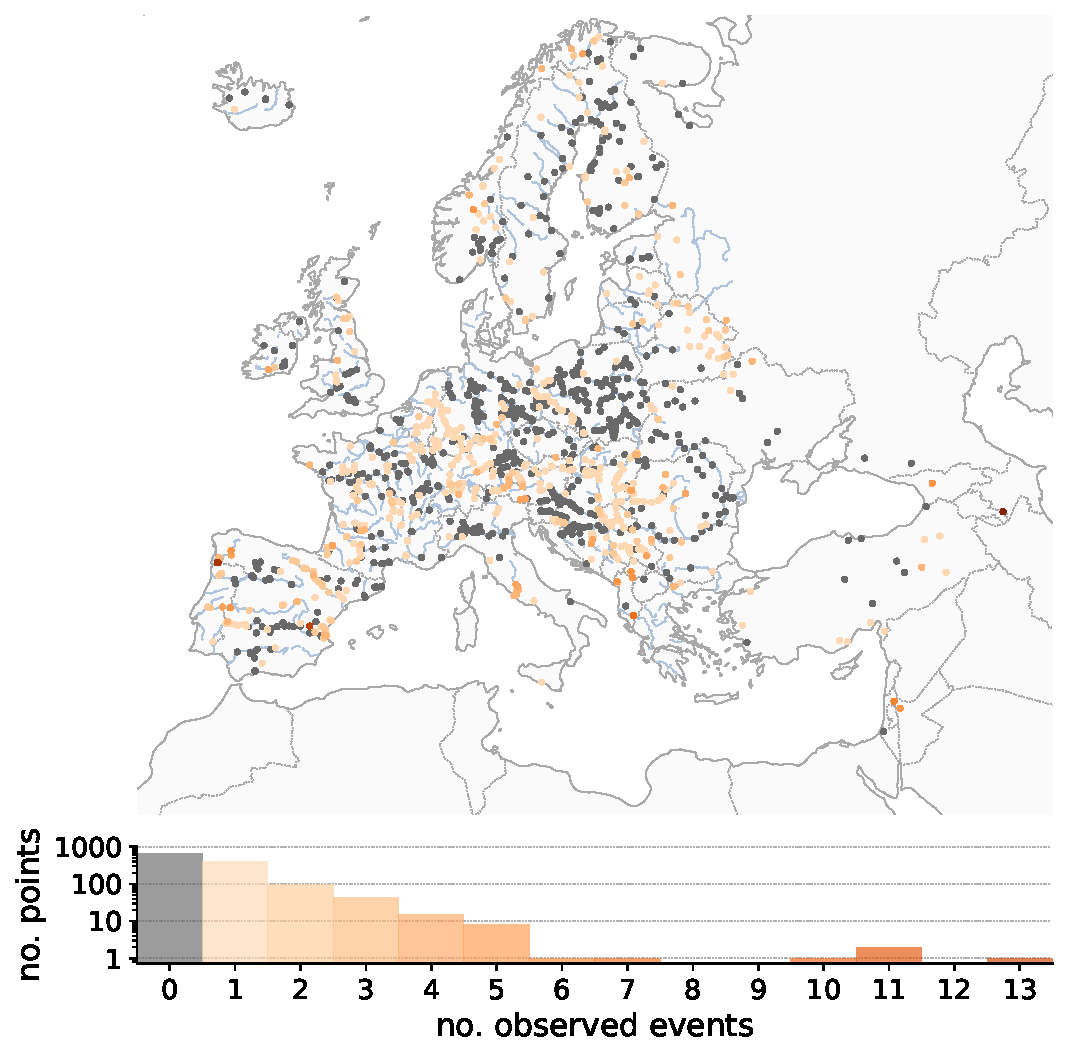
\includegraphics[width=0.75\linewidth]{figures/map_observed_events_2000km2_1239points.pdf}
    \caption{Geographical distribution of the stations used for optimizing the notification criteria, and number of "observed" flood events during the study period.}
    \label{fig:map_observed}
\end{figure}

In total, the optimization of the notification criteria will be based on 1239 stations and 874 "observed events". A higher concentration of points with events is observed in Central Europe, the British Isles, and Mediterranean catchments. Significant flood events in the Rhine, Meuse, and Ebro are visually evident on the map. Throughout the study period, 61\% of the stations did not exceed the 5 year return period. For this proportion of the sample, predicting hits or misses is not possible, and the only term in the contingency table will be false alarms. Consequently, the f-score for these points may be either nonexistent or 0. Additionally, 29\% of stations registered only one "observed" event, resulting in f-score possibilities of either 0 or 1. These nuances bear implications for the overall skill of the system, as we will explore in subsequent discussions. 

The imposition of a minimum contributing area of 2000 km² places a constraint on the number of stations available for optimization, consequently affecting the count of observed events. In the final phase of our analysis, we will assess the implications of this criterion by expanding our consideration to stations with a minimum area of 500 km². Figure \ref{fig:observed_vs_area} represents the relationship between the increasing catchment area threshold and the corresponding number of stations and "observed" events. Both counts decrease exponentially with catchment area. By excluding the points with contributing area smaller than 2000 km², we discard 37\% of the stations and 48\% of the events.

\begin{figure}
    \centering
    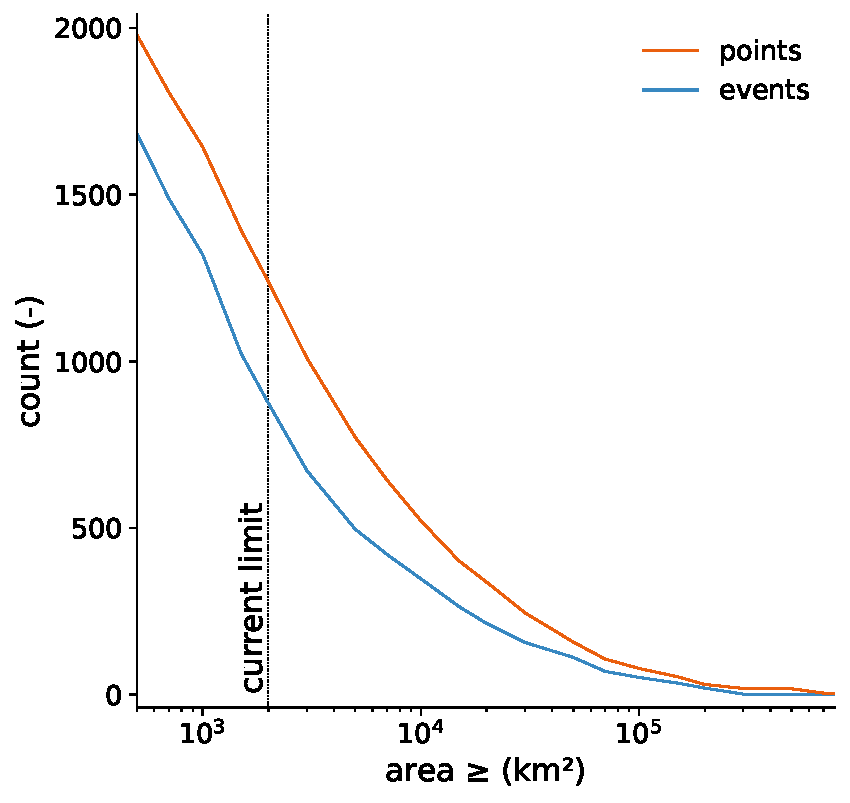
\includegraphics[width=0.5\linewidth]{figures/points_observedEvents_vs_area_2000km2_1239points.pdf}
    \caption{Number of stations (orange) and observed events (blue) by catchment area threshold. The vertical, dotted line represents a catchment area of 2000 km², the current limit in the notifications.}
    \label{fig:observed_vs_area}
\end{figure}

\subsection{Individual NWP}
\label{sec:results_NWP}

Prior to studying how to combine the NWP models, we analysed the skill of each of the models individually. This analysis serves a dual purpose. First, to understand the relative skill of each model, with the intention of incorporating this skill into the computation of the total probability. Second, to compare the skill  of individual NWP models against the benchmark— the current notification criteria—, and to set a baseline for the combination methods.

\subsubsection{Probabilistic skill}
\label{sec:NWP_prob_skill}

In the initial assessment of NWP skill, we calculated the Brier score for each NWP at daily lead times. The Brier score, as an error metric, yields values that can be challenging to interpret, given the dependence of error magnitude on the specific variable—particularly in the context of rare events like floods, where the magnitude is inherently low. Instead, we employ the Brier skill score (BSS) to gauge the relative skill of a model in comparison to a reference. Models outperforming the reference receive a positive BSS, while those underperforming register a negative BSS. For the reference, we opted for a dummy model that never predicts an event ($P_{pred}=0$) \cite{Legg2004}.

\begin{figure}
    \centering
    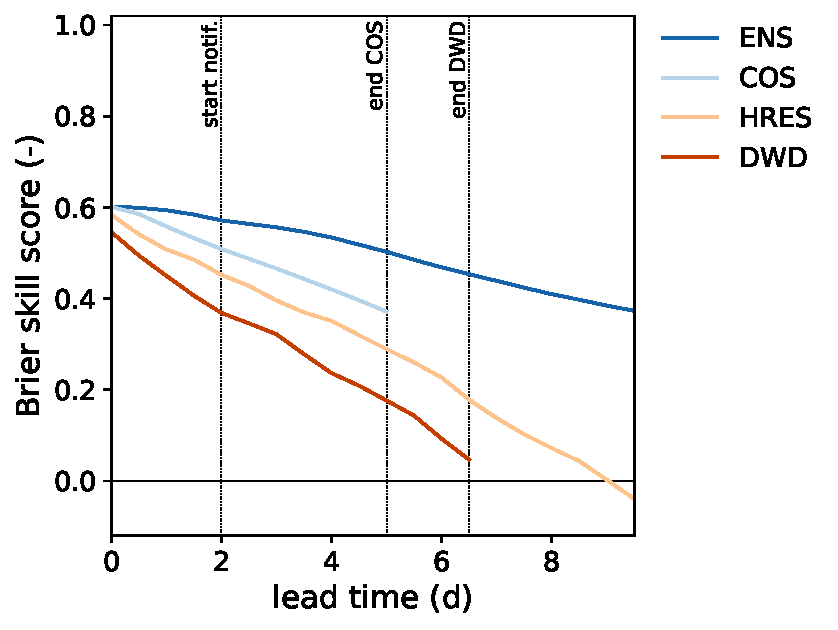
\includegraphics[width=0.5\textwidth]{figures/Brier_skill_score_5.pdf}
    \caption{Brier skill score of the four NWP used in EFAS at daily lead times. The reference ($BSS=0$) is a model that never predicts an event. Blue lines represent probabilistic models, and orange lines deterministic ones.}
    \label{fig:BSS}
\end{figure}

The plot above demonstrates that probabilistic models exhibit greater skill than deterministic ones. Only within very short lead times (0-1 days) do deterministic models approach the skill observed in probabilistic models. This is particularly significant for EFAS notifications, as the formal notifications are reserved for lead times greater than 2 days (indicated by  the leftmost dotted line). 

As lead time increases, there is a degradation in skill. This decline impacts ENS to a lesser extent than the other models. Both deterministic models display poor skill at their forecast horizon. For instance, at 10 days lead time, the skill of HRES is worse than a model that never predicts a flood. 

Overall, the most skillful model for flood warning forecasting is ENS, while the least skillful is DWD. In section \ref{sec:results_COMB}, we will convert the Brier into weighing factors for the computation of total probability (see Figure \ref{fig:weights}).

\subsubsection{Notification skill}
\label{sec:NWP_skill}

In this section we analysed how the NWP would have performed if notifications would be sent based uniquely in one of them. First, we want to have a general picture of how notification skill evolves according to the 3 dimensions here involved (lead time, probability threshold and persistence). Second, we will optimize the probability and persistence criteria for a fixed lead time.

Figure \ref{fig:NWP_skill_leadtime} exhibits the evolution of the notification skill with lead time and probability threshold for a scenario with no persistence. The black, solid line is the notification skill of the current notification criteria, as a benchmark to compare the skill of the individual NWP models. Each colour line represents a different probability threshold; orange lines represent thresholds below 50\% and blue lines over that value. For the two deterministic models (DWD, HRES) all lines overlap, since the probability threshold does not affect a deterministic forecast.

\begin{figure}
    \centering
    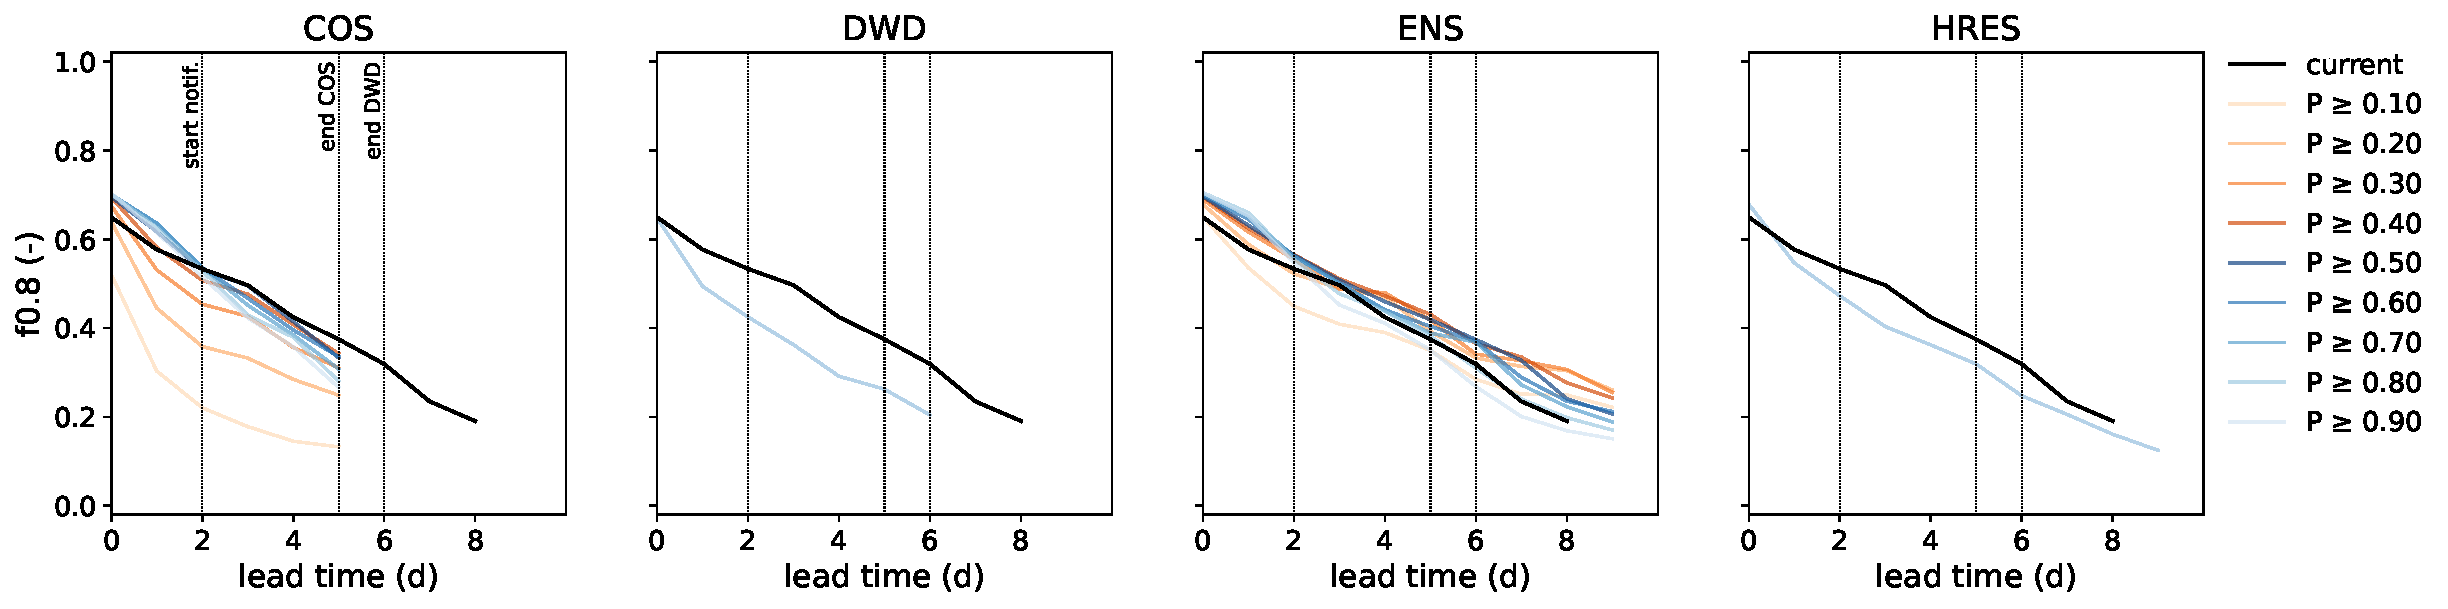
\includegraphics[width=1\textwidth]{figures/skill_probability_leadtime_1-1_NWP.pdf}
    \caption{Evolution of the notification skill with daily lead times and probability threshold for each NWP model in an scenario with no persistence. Each plot represents a different NWP. As a benchmark, the black, solid line represents the skill of the current operational criteria (1 deterministic + 1 probabilistic, 30\% probability and a persistence of 3 forecasts).}
    \label{fig:NWP_skill_leadtime}
\end{figure}

In line with Figure \ref{fig:BSS}, the probabilistic models are more skillful than the deterministic. Under some conditions, they even outperform the current notification criteria, which means that there is ground for improving the skill of the current EFAS notification criteria. Deterministic models are as skillful as the current criteria only for the very first lead time.

As expected, notification skill degrades with lead time. This applies to all cases (deterministic, probabilistic and benchmark), but the rate of degradation is affected by the probability threshold. Low probability thresholds degrade sharply at short lead times, and high probability thresholds have a larger loss of skill at long lead times (see ENS over 7 days). 

There is a range of probability thresholds from approximately 40\% to 80\% with similar good skill. Within this range, larger thresholds perform slightly better at short lead times, and lower thresholds perform slightly better at mid-long lead times. Since we need to find out a single probability threshold for the notification criteria, the selection of the optimal criteria will focus on a lead time range from 2 days (the minimum formal notification lead time) to 5.5 days (the maximum lead time in COS). In this range we avoid the large uncertainty at long lead times and we focus on the lead times at which the majority of the formal notifications are issued.

So far, we have removed persistence from the exploration. To evaluate the effects of persistence in the notification skill we have produced the plot in Figure \ref{fig:NWP_skill_probability}, which shows the evolution of skill with the probability threshold and persistence for a fixed lead time range (2-5.5 days). The benchmark (current notification criteria) is now a single point corresponding the 30\% probability and persistence 3/3. As the probability threshold does not affect deterministic forecasts, the lines for the two deterministic models (DWD and HRES) are horizontal.

\begin{figure}
    \centering
    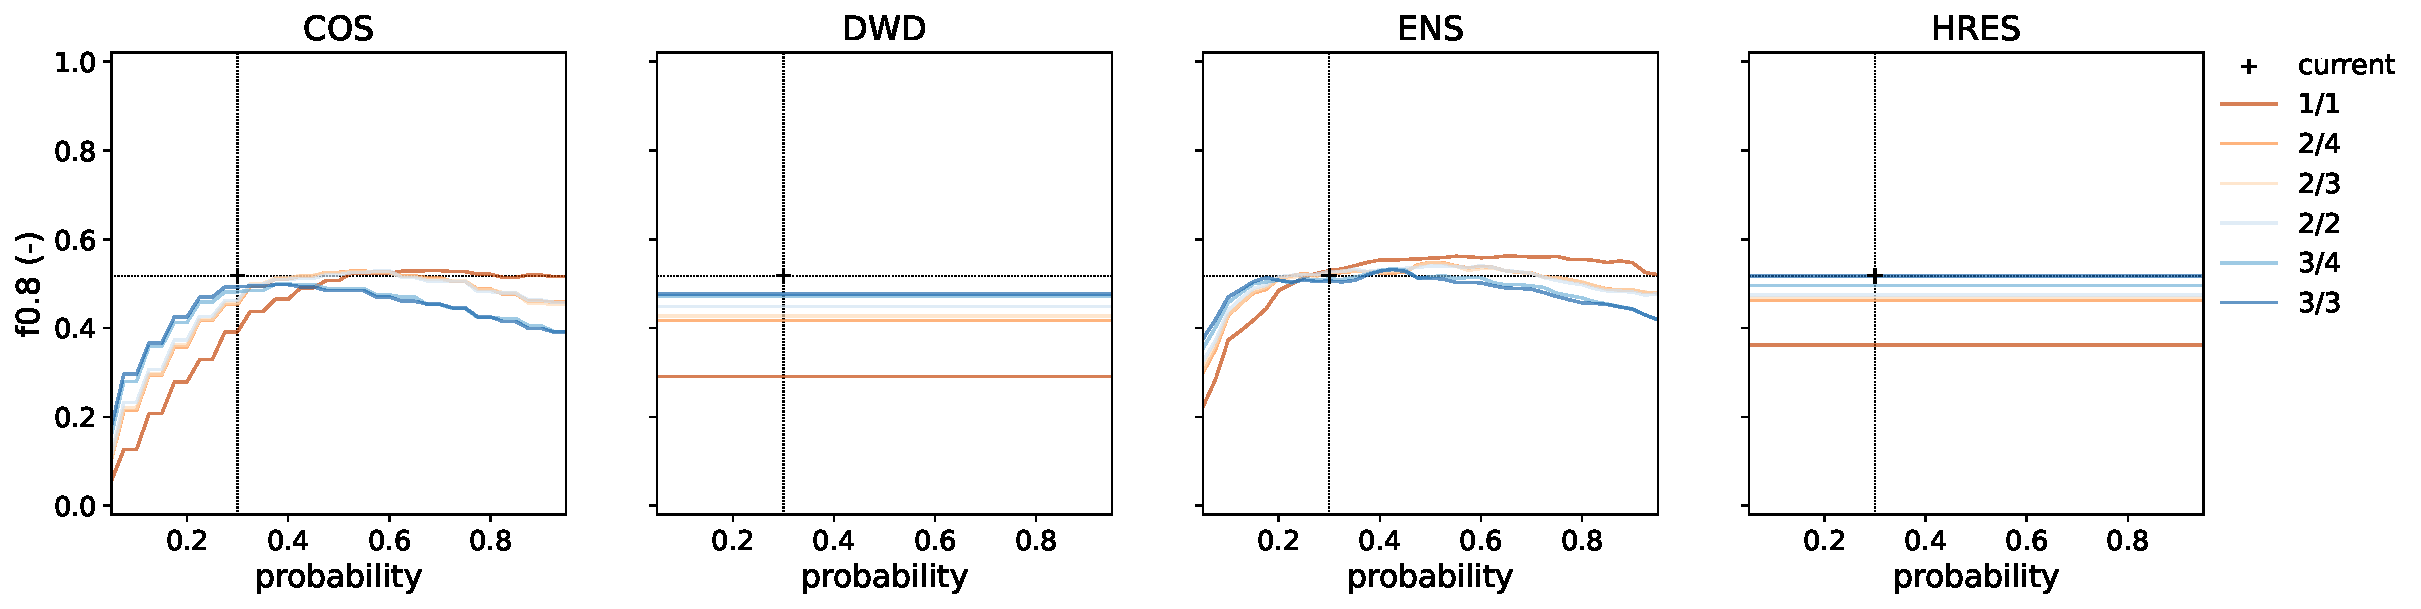
\includegraphics[width=1\textwidth]{figures/skill_persistence_probability_060h_NWP.pdf}
    \caption{Evolution of the notification skill with probability threshold and persistence  for each NWP model at a fixed lead time range (from 2 to 5.5 days). Each plot represents a different NWP model. As a benchmark, the black dot represents the current criteria (1 deterministic + 1 probabilistic, 30\% probability and a persistence of 3 forecasts).}
    \label{fig:NWP_skill_probability}
\end{figure}

Three out of four NWP models are able to replicate or improve the skill of the current notification criteria at some combinations of persistence and probability. Only DWD is less skillful than the benchmark.

The skill of the probabilistic models shows a trade-off between probability threshold and persistence. Both criteria play the same role, which is removing false positives (or uncertain events) by taking stricter values. Hence, increasing values of persistence require lower probability thresholds to optimize the skill. Nevertheless, the scenario of no persistence produces the highest notification skill. At this scenario, there is a wide range of probability thresholds (from 40/50\% to 90\%) that perform similarly good.

Persistence does make a larger difference in the deterministic models. Their skill improves dramatically as soon as some persistence is added in the criteria. For the most stringent persistence (3/3), the skill of the deterministic HRES is as good as that of the probabilistic ENS, and even better than COSMO-LEPS. However, as explained earlier, this is a sub-optimal set of criteria; it does not outperform the probabilistic models with no persistence.

With the knowledge gained in the previous exploration, we were in a better position to optimize the notification criteria and understand the results. Table 1 summarizes the results of the optimization of notification criteria for the individual NWP models. The results are organised by lead time ranges; for each range, the table presents the optimized criteria (probability and persistence) and the skill metrics (recall, precision and f0.8) for the available NWP models. As a benchmark, the first row in each lead time range shows the skill of the current operational criteria. The objective of the optimization is two-fold: first, to compare the optimal skill of the different NWPs, second, to set a baseline against which we can assess the added value of combining all NWPs.

\begin{table}
    \centering
    \caption{Summary of the optimization of the notification criteria for individual NWP and four lead time ranges. Skill metrics refer to the complete set of stations.  The initial row serves as a benchmark, indicating the skill of the current notification criteria. In each lead time range, bold figures highlight the peak value for a specific metric.}
    \footnotesize
    \begin{tabular}{cccccccc}
        \toprule
        lead time & model & probability & persistence & recall & precision & $\text{f}_{0.8}$ & rank \\
        \midrule
        \textless 2 d & 1D+1P & 0.300& 3/3 & 0.522 & \textbf{0.735} & 0.634 & 3 \\
         & COS & 0.875 & 1/1 & 0.673 & 0.718 & \textbf{0.700} & 1 \\
         & DWD & - & 2/2 & 0.585 & 0.583 & 0.583 & 5 \\
         & ENS& 0.800 & 1/1 & \textbf{0.681} & 0.711 & 0.699 & 2\\
         & HRES& -& 2/2 & 0.580 & 0.671 & 0.632 & 4\\
         \midrule
        2-5.5 d & 1D+1P & 0.300& 3/3 & 0.413 & 0.618 & 0.518 & 3 \\
         & COS & 0.725 & 1/1 & 0.387 & 0.687 & 0.518 & 2 \\
         & DWD & - & 3/3 & \textbf{0.420} & 0.522 & 0.477 & 5 \\
         & ENS & 0.650 & 1/1 & 0.416 & \textbf{0.725} & \textbf{0.562} & 1 \\
         & HRES & - & 3/3 & 0.416 & 0.612 & 0.517 & 4 \\
         \midrule
        5.5-7 d & 1D+1P & 0.300& 3/3 & 0.215 & \textbf{0.612} & 0.356 & 2 \\
         & DWD & - & 2/2 & \textbf{0.291} & 0.358 & 0.328 & 4 \\
         & ENS & 0.450 & 1/1 & 0.264 & 0.605 & \textbf{0.402} & 1 \\
         & HRES & - & 2/2 & 0.273 & 0.429 & 0.351 & 3 \\
         \midrule
        7-10 d & 1D+1P & 0.300& 3/3 & 0.120 & \textbf{0.625} & 0.237 & 3 \\
         & ENS & 0.175 & 2/2 & \textbf{0.287} & 0.396 & \textbf{0.345} & 1 \\
         & HRES & - & 2/2 & 0.244 & 0.336 & 0.293 & 2 \\
         \bottomrule
    \end{tabular}
    \label{tab:NWP_optimization}
\end{table}

When looking at the f-score, the current notification criteria (1D+1P) are outperformed at any lead time range by at least one NWP. If we focus in the lead time range from 2 to 5.5 days, the current criteria are able to notify 41\% of the events (recall) and 62\% of the notifications are correct (precision). The current criteria seem too strict, i.e., notifications are issued only with a high level of certainty. Whenever sent, they turn out to be mostly correct, but many events are missed. If we turn this values into skill (see Table 1), the current criteria  has an $f_{0.8}$ score of 0.518.

For the first lead time range, the best NWP is COS, with ENS showing almost equal skill. Both ENS and COS optimized a very high probability threshold and persistence was not required. The skill of the 2 deterministic NWP is distinctively lower, especially in the case of DWD. The 2 models optimized a persistence of 2/2. When comparing the skill of individual NWP with the current operational criteria, we find out that any of the 2 probabilistic models independently outperform the current criteria, and the deterministic HRES almost reaches the benchmark skill.

The picture does not change when looking at lead times from 2 to 5.5 days. The 2 probabilistic NWP have a higher skill than the deterministic ones and outperform the current operational criteria, but in this case ENS is the best NWP. Neither of the probabilistic models require persistence and the probability thresholds are lower than in the previous lead time range, but still higher than the 30\% value used currently. Again the deterministic models require a persistence of 3, and HRES almost equals the benchmark skill. Overall, there is a loss in skill of approximately 20\% compared with the first 2 days of forecast. 

For lead times from 5.5 to 7 days COS is not available any more. The only probabilistic model, ENS, outperforms the deterministic models and the benchmark. The probability threshold optimized for this lead time range is lower than in shorter lead times, but still larger than the current operational value. In general, there has been a loss in skill of approximately 30\% with respect to the previous lead time range (above 40\% compared with the first 2 days of forecast).

In the last 3 days of forecast only ENS and HRES are available. Both of the NWP models outperform the current criteria, but ENS is clearly more skillful than HRES. This long lead time range is the only one for which ENS required persistence (2/2), whereas the probability threshold is slightly lower than in the previous range.

Comment the Roebber diagram!!! Negatively biases, i.e., EFAS produces less notifications that the number of actual events.

\begin{figure}
    \centering
    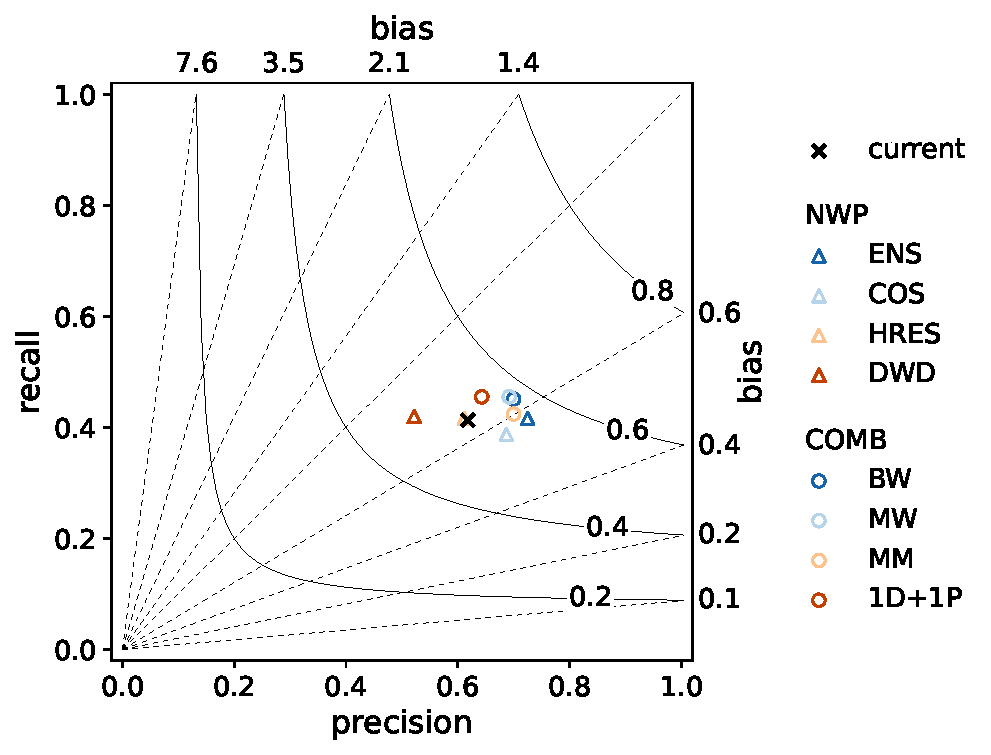
\includegraphics[width=0.5\linewidth]{figures/roebber_fscore_60h.pdf}
    \caption{Roebber diagram of the optimized criteria at the lead time range from 2 to 5.5 days. Triangles represent individual NWP and circles the 4 combination of NWP tested in this work. As a reference, the skill of the current notification criteria is been added as a black cross. The Roebber diagram shows in a single plot 4 skill metrics: precision and recall in the X and Y axis, bias is represented by the dashed lines, and the $f_{0.8}$ score by the solid lines.} 
    \label{fig:roebber}
\end{figure}

\subsection{Combination of models}
\label{sec:results_COMB}

Three of the four combination methods compute total probability. To do so weights need to be assigned to every NWP. Figure \ref{fig:weights} shows the distribution of weights among NWP models for those three combination methods, and how the weights change with lead time.

\begin{figure}
    \centering
    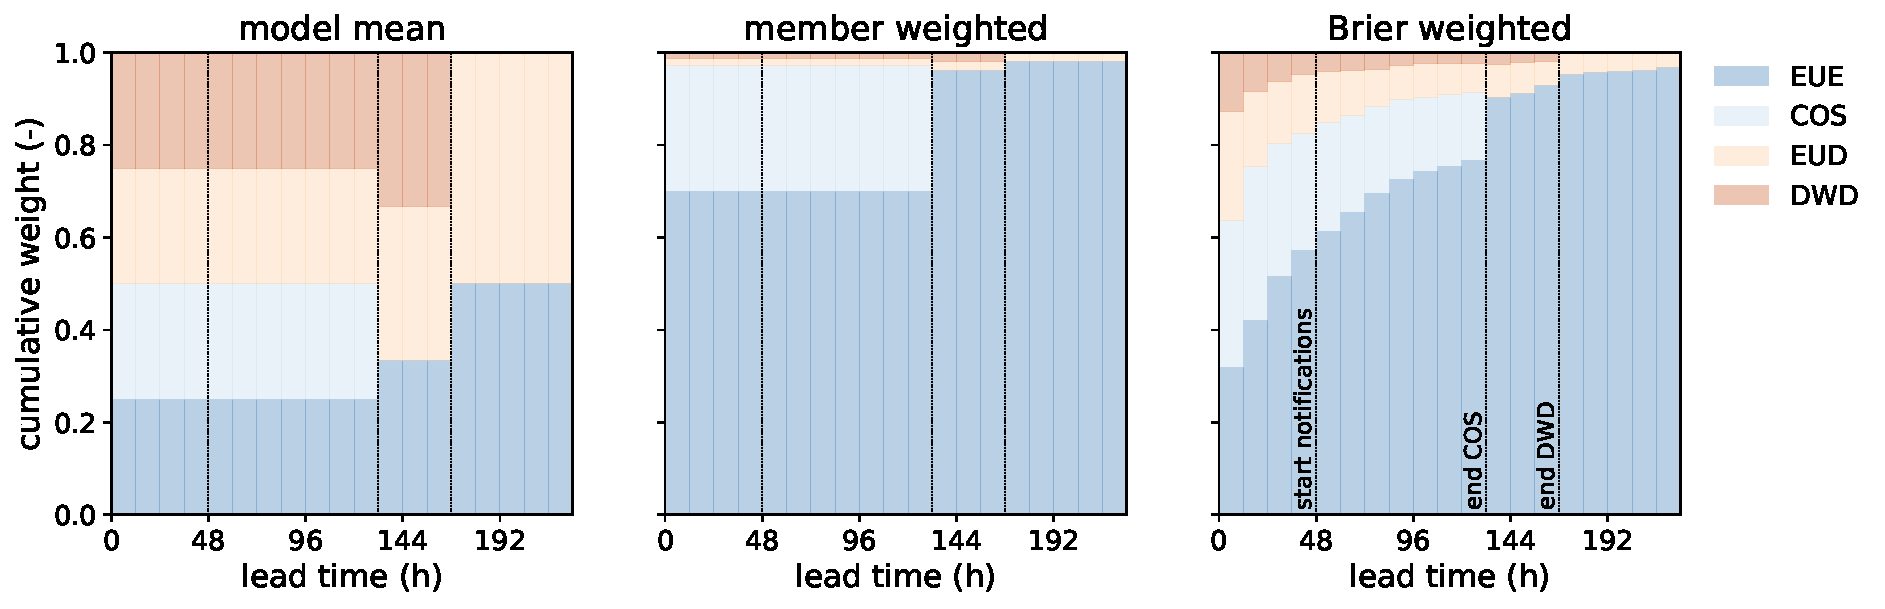
\includegraphics[width=1\textwidth]{figures/weights.pdf}
    \caption{Weights applied to compute the total probability out of the NWP models. Every plot represents a different approach. Colours represent the NWP (blue for probabilistic and orange for deterministic models).}
    \label{fig:weights}
\end{figure}

The model mean (MM) approach attributes equal weights to each model. The changes in the weights with lead time occur when the maximum lead time of a model is exceeded (5.5 days for COS and 7 days for DWD). This is the approach in which the deterministic models are given the same importance as the probabilistic models.

In the member weighted (MW) combination, every model run is assigned an equal weight. Therefore, ENS, which has a significant larger number of members, prevails over any other NWP. Even for the first 5 days, when all the models are available, ENS gets 70\% of the weight. Instead, the sum of the two deterministic models (HRES and DWD) has a maximum weight of 4\% from days 5.5 to 7. If we compare these weights to the current 30\% probability criterion, it means that in the case that ENS completely fails to predict an event, the 30\% total probability could never be achieved at lead times longer than 5.5 days, and only if all the other models were completely correct would the event be notified at lead times shorter than 5.5 days. In general, this approach relies heavily on the skill of ENS, which fortunately is the most skillful model (see Figure \ref{fig:BSS}).

In the Brier weighted (BW) combination, the Brier score values from section \ref{sec:NWP_prob_skill} were transformed to be used as weighing factors in the computation of the total probability. This transformation consisted of re-scaling the original values by inverse distance weighing, so that the sum of all weights is 1. The resulting weights vary with lead time, showing a transition from short to long lead times. At very short lead times the deterministic models are skillful, so they sum up to a third of the weight. As the lead time increases, the probabilistic models, especially ENS, take most of the weight. At lead times from 2 to 5.5 days, when most of the notifications are sent, the probabilistic models carry at least 80\% of the weight.

\subsubsection{Notification skill}
\label{sec:COMB_skill}

Figure \ref{fig:COMB_skill_leadtime} and Figure \ref{fig:COMB_skill_probability} replicate the analysis of the notification skill previously done for the individual NWP models, but this time for the combination methods. Figure \ref{fig:COMB_skill_leadtime} shows the evolution of the notification skill with lead time and probability threshold for a fixed persistence value (no persistence). Figure \ref{fig:COMB_skill_probability} presents, instead, the evolution with probability and persistence for a fixed lead time range (2-5.5 days). Together they portray an overall picture of the behaviour of skill in the four dimensions: combination method, lead time, probability threshold and persistence.

\begin{figure}
    \centering
    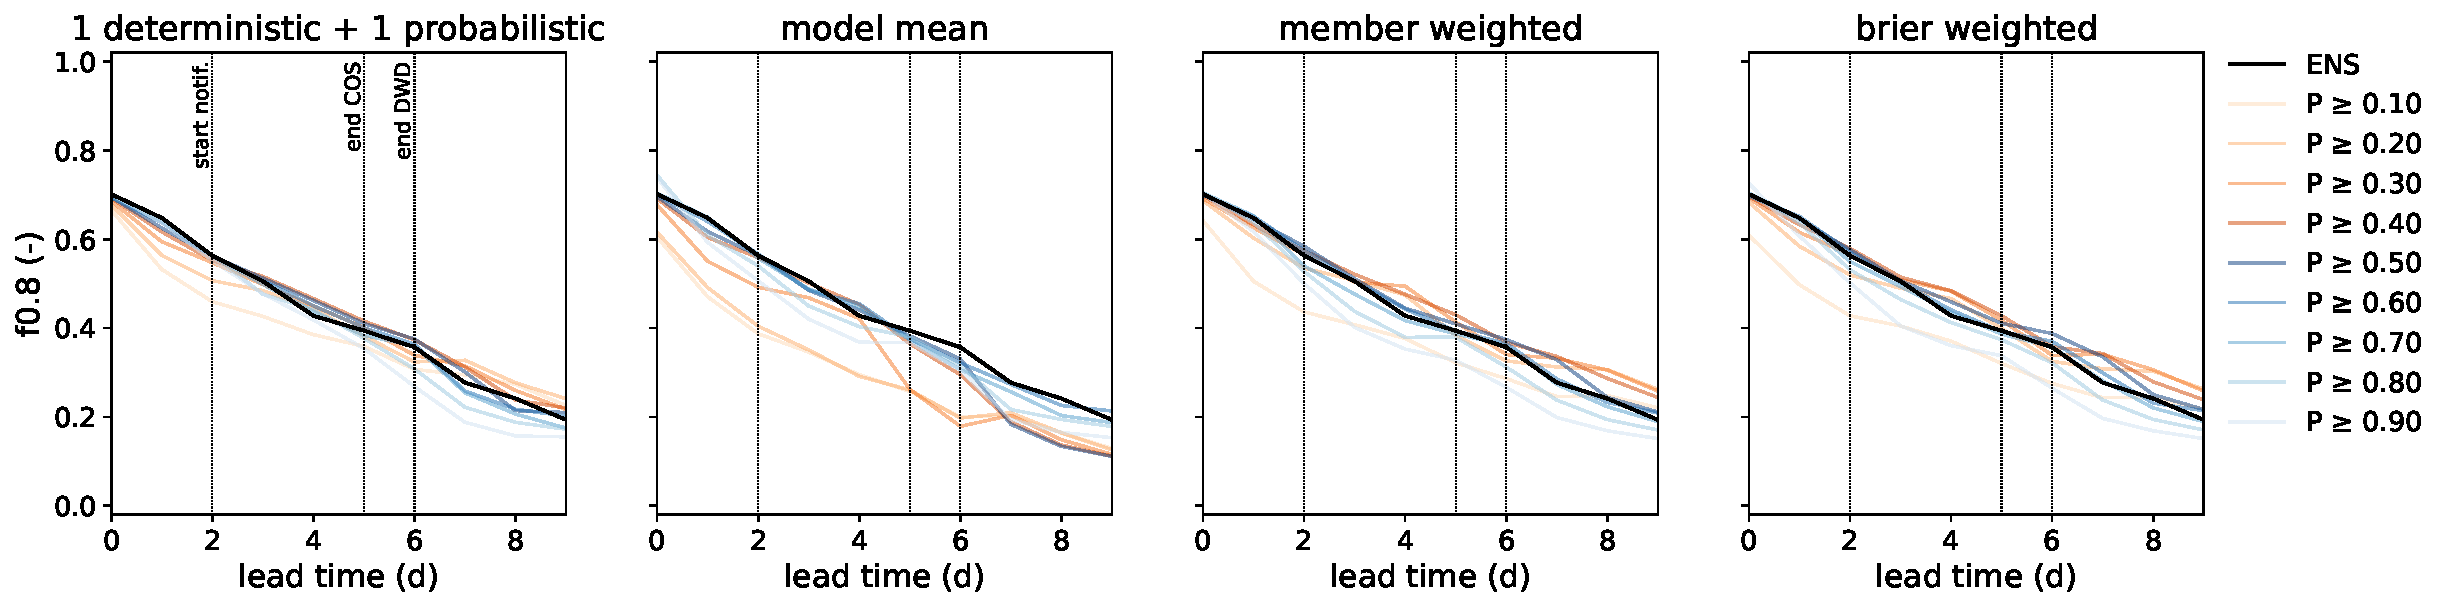
\includegraphics[width=1\textwidth]{figures/skill_probability_leadtime_1-1_COMB_vs_ENS.pdf}
    \caption{Evolution of the notification skill with daily lead times and probability threshold for each of the combination methods in an scenario with no persistence. Each plot represents a different combination of NWP. As a benchmark, the black, solid line represents the skill of ENS with optimized criteria (65\% probability and no persistence).}
    \label{fig:COMB_skill_leadtime}
\end{figure}

As ENS is the most skillful NWP, using it as a benchmark establishes  a tough competition. Three out four of combinations (1D+1P, MW, BW) are capable of adding value to the ENS benchmark, but only from lead time 4 onward. In any case, the improvement in skill is limited. The skill among combinations is fairly similar, but we can already notice that the member weighted  and Brier weighted  approaches slightly outperform the other two. Except for the model mean, larger probability thresholds perform better at short lead times and smaller thresholds at longer lead times. Despite that fact, there is equifinality in the optimum of the probability thresholds. This behaviour of the probability threshold was already seen in the individual NWP.

Regardless of the NWP or combination of NWP, the notification skill degrades notably with lead time. Even if at lead time 0 the skill is high (up to 0.74), the minimum lead time criterion limits the EFAS notification skill to values slightly lower than 0.6. The degradation continues and, from day 7 onward, the skill drops below 0.4, which may be an indicator for creating a new limitation on the maximum lead time at which notifications are issued.

\begin{figure}
    \centering
    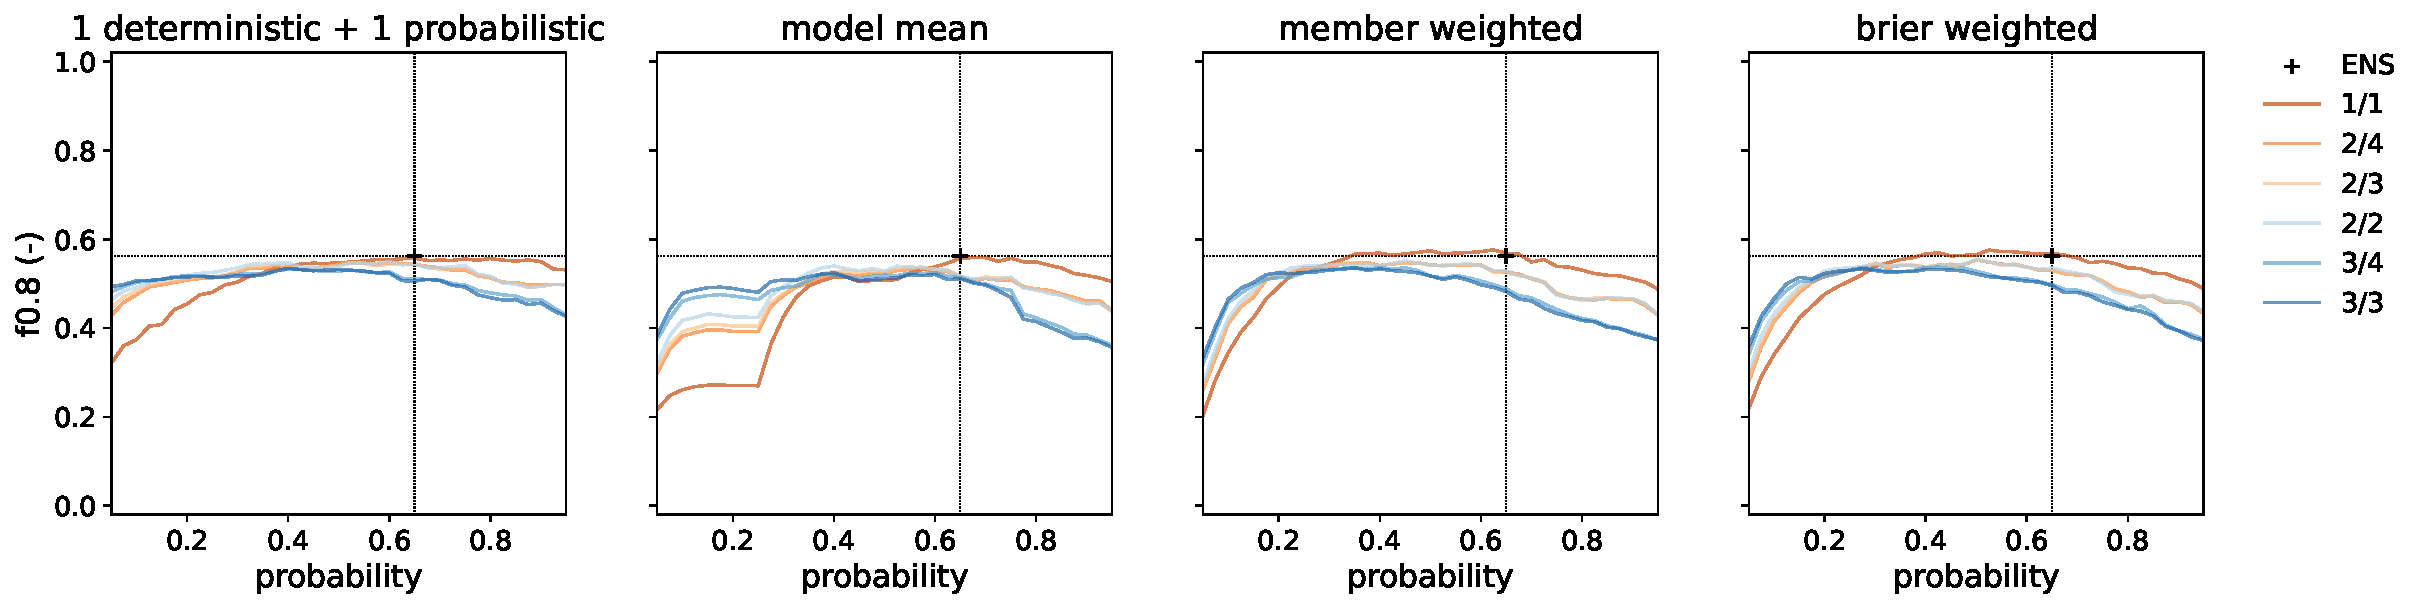
\includegraphics[width=1\textwidth]{figures/skill_persistence_probability_060h_COMB_vs_ENS.pdf}
    \caption{Evolution of the notification skill with probability threshold and persistence  for each combination of NWP at a fixed lead time range (from 2 to 5.5 days). Each plot represents a different NWP model. Each plot represents a different combination of NWP. As a benchmark, the black cross represents the skill of ENS with optimized criteria (65\% probability and no persistence).}
    \label{fig:COMB_skill_probability}
\end{figure}

Figure \ref{fig:COMB_skill_probability} proves that introducing the persistence criterion limits the maximum attainable skill. Across all four combinations, the highest skill is reached when no persistence is applied (1/1). In this scenario, all combinations exhibit similar maximum skill. Only member weighted (MW) and Brier weighted  (BW) marginally surpass the baseline (ENS). These two combinations show optimal skill within a range of probability thresholds spanning 40\% to 70\%. In both instances, the maximum skill is achieved at a probability threshold lower than that optimized for ENS.

The absence of sensitivity to probability in the current criteria (indicated by the dark blue line in the left-hand side pane) is noteworthy. Even at the lowest probability threshold, the f0.8 score remains at 0.5, unlike other approaches where there is a significant decline in performance as the probability threshold approaches very low values.

Table 2 summarizes the results of the optimization of the notification criteria for the combination methods in an identical way as Table 1 did for the NWP. The results are organised by lead time ranges; for each range, the table presents the optimized criteria (probability and persistence) and the skill metrics (recall, precision and f0.8) for the four methods. As a baseline, the first row in each lead time range shows the skill of ENS, which we established as the reference NWP in Table 1. The objective of the optimization is again two-fold: to compare the four combinations of NWP models, and to assess the added value of combining all NWPs instead of simply using the baseline. 

\begin{table}
    \centering
    \caption{Summary of the optimization of the notification criteria for the combination methods and four lead time ranges. Skill metrics refer to the complete set of stations. The initial row serves as a baseline, indicating the skill of ENS, the top-performing NWP. In each lead time range, bold figures highlight the peak value for a specific metric. }
    \footnotesize
    \begin{tabular}{cccccccc}
        \toprule
        lead time & method & probability & persistence & recall & precision & $f_{0.8}$ & rank \\
        \midrule
        \textless 2 d& ENS & 0.800 & 1/1 & \textbf{0.681} & 0.711 & 0.699 & 4 \\
         & 1D+1P & 0.925 & 1/1 & 0.662 & 0.717 & 0.694 & 5 \\
         & MM & 0.775 & 1/1 & 0.628 & \textbf{0.838} & \textbf{0.741} & 1 \\
         & MW & 0.750 & 1/1 & 0.673 & 0.718 & 0.700 & 3 \\
         & BW & 0.950 & 1/1 & 0.620 & 0.829 & 0.733 & 2 \\
         \midrule
        2-5.5 d & ENS & 0.650 & 1/1 & 0.416 & \textbf{0.725} & 0.562 & 3 \\
         & 1D+1P & 0.600 & 1/1 & \textbf{0.455} & 0.643 & 0.554 & 5 \\
         & MM & 0.700 & 1/1 & 0.424 & 0.700 & 0.559 & 4 \\
         & MW & 0.500 & 1/1 & \textbf{0.455} & 0.692 & 0.574 & 2 \\
         & BW & 0.525 & 1/1 & 0.451 & 0.700 & \textbf{0.576} & 1 \\
         \midrule
        5.5-7 d & ENS & 0.450 & 1/1 & 0.264 & \textbf{0.605} & \textbf{0.402} & 1 \\
         & 1D+1P & 0.425 & 1/1 & 0.262 & 0.599 & 0.399 & 4 \\
         & MM & 0.500 & 1/1 & \textbf{0.276} & 0.412 & 0.345 & 5 \\
         & MW & 0.425 & 1/1 & 0.271 & 0.579 & 0.401 & 2 \\
         & BW & 0.450 & 1/1 & 0.268 & 0.586 & 0.400 & 3 \\
         \midrule
        7-10 d & ENS & 0.175 & 2/2 & \textbf{0.287} & 0.396 & \textbf{0.345} & 1 \\
         & 1D+1P & 0.250 & 1/1 & 0.256 & 0.414 & 0.334 & 4 \\
         & MM & 0.225 & 2/2 & 0.252 & 0.334 & 0.296 & 5 \\
         & MW & 0.175 & 2/2 & 0.278 & 0.402 & 0.343 & 3 \\
         & BW & 0.300 & 1/1 & 0.255 & \textbf{0.445} & \textbf{0.345} & 1 \\
         \bottomrule
    \end{tabular}
    \label{tab:COMB_optimization}
\end{table}

In the shortest lead time range, two combinations clearly outperform the baseline (MM, BW). Between the two, MM exhibits the highest skill ($f_{0.8}=0.741$). This proficiency can be attributed to MM emphasis on deterministic models, which demonstrated notable skill at very short lead times (see Figure \ref{fig:weights}). As of the optimized criteria, none of the four methods required persistence, and probability thresholds fell within the top quartile. At this lead time range EFAS formal notifications are not issued, so the results above are only informative, but do not affect the selection of new criteria.

From day 2 to 5.5, BW and MW stand out as the top-performing combinations, showcasing comparable skill that surpass the baseline. Both approaches operate optimally without the need for persistence, with the probability threshold hovering around 50\% (refer to Figure \ref{fig:COMB_skill_probability} for a sense of the uncertainty in defining the probability threshold). Compared with the preceding lead time range, there is an evident decline in skill by approximately 20\%. This is the lead time range at which most of the notifications are issued, so the decision about the new notification criteria will be based on this results.

In the third lead time range, from 5.5 to 7 days, none of the combinations outperform the baseline, despite three of them (1D+1P, MW and BW) attaining very similar skill. None of these three methods necessitated the use of persistence, and the associated probability thresholds were slightly lower than those in the preceding lead time range (around 40\%). When compared with the prior lead time range, there is a decrease in skill of around 30\% (45\% when compared to the the first range).

In the longest lead time range, BW emerges as the best-performing combination, with a skill on par with the baseline. MW, while slightly less proficient, shows similar skill. However, their optimized criteria differ. MW requires a persistence of 2 out of 2 forecasts and a relatively low probability threshold (0.175) — precisely the same criteria optimized for the baseline. In contrast, BW does not require persistence, and its probability threshold (30\%) aligns with the decreasing trend observed in previous lead time ranges.

The maps in Figure \ref{fig:maps_BW} illustrate the skill metrics associated with the optimal notification criteria, i.e., the BW combination with no persistence and a probability threshold of 52.5\%. The metrics represent only the lead time range from 2 to 5.5 days, which corresponds to the period when the majority of the notifications are issued. 

\begin{figure}
    \centering
    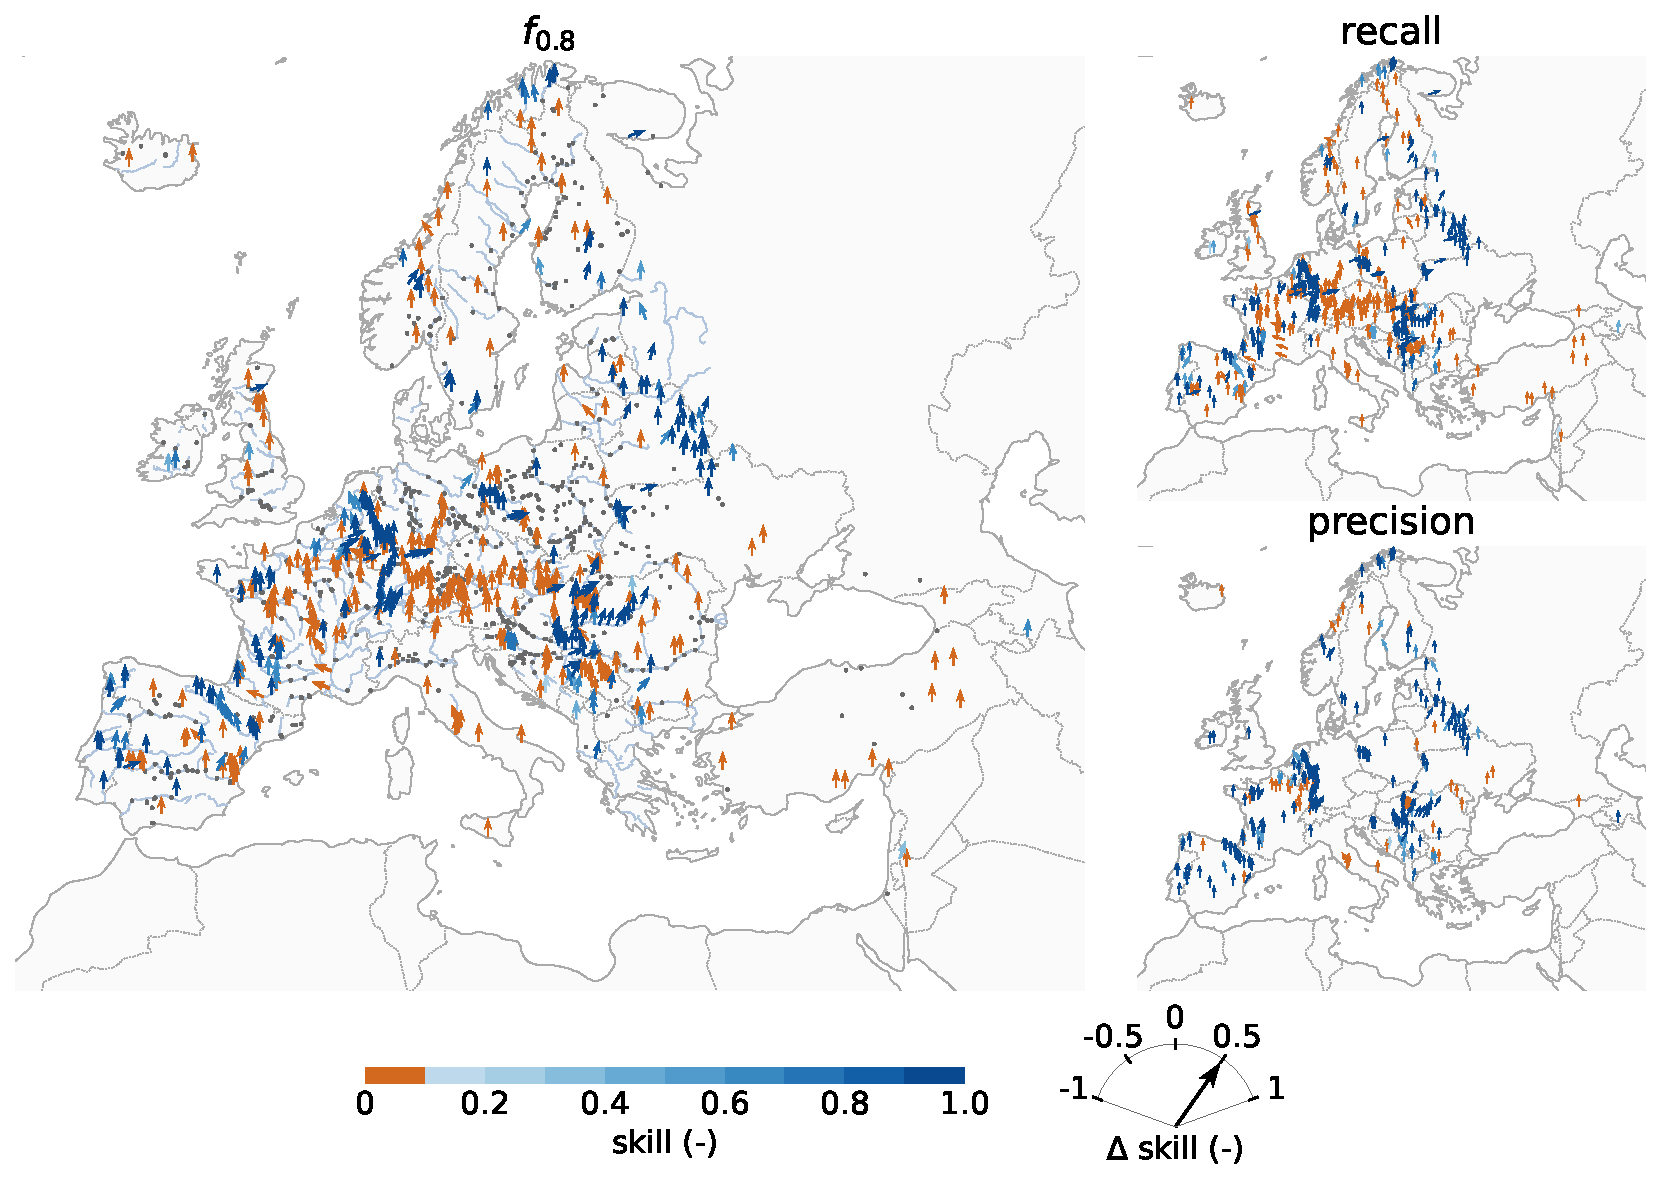
\includegraphics[width=1\linewidth]{figures/skill_maps_reporting_points_2000km2_1239points_brier_weighted_060h_arrows.pdf}
    \caption{Skill maps for the optimized notification criteria (BW, 52.5\% probability threshold and no persistence) at the lead time range from 2 to 5.5 days. The main plot shows the skill in terms of $f_{0.8}$ (the target metric); in this plot, gray dots are stations for which the f-score cannot be computed due to all instances of hits, misses and false alarms being null. The smaller plots show precision and recall, the components of the f-score; for the sake of visibility, it only shows the stations for which the specific metric can be computed. In all the plots the direction of the arrows shows the difference in that metric between the optimized criteria and the current criteria, i.e., positive values imply gains and negative values losses in skill.}
    \label{fig:maps_BW}
\end{figure}

A pronounced contrast is evident in the maps, attributable to the limited number of events in most stations, resulting in skill metrics primarily yielding values of either 1 or 0 . In terms of f-score, there is a clustering of underperforming points in central Europe (notably the Alps) and central France. The breakdown into recall and precision reveals that the predominant cause of the low f-score lies in recall, indicating missed events. Conversely, the precision of notifications remains consistently high, with exceptions observed in the Seine and Arno rivers. It is noteworthy the skill in all metrics for the Ebro, Rhine and Meuse—three rivers that experienced significant flood events during the study period.

Applying this set of criteria would enable EFAS to notify 45\% of the events, and 70\% of the notifications would be correct. For reference, these figures represent a improvement in both metrics over the existing criteria, which achieved 41\% recall and 62\% precision (see Figure \ref{fig:roebber}).

\subsection{Skill by catchment area}
\label{sec:skill_area}

The preceding sections present results for a set of stations with a catchment area of at least 2000 km², the current limit. To investigate the potential relaxation of this criterion, Figure \ref{fig:skill_area} illustrates the evolution of skill depending on the catchment area limit. The criteria used to create this figure are those optimized for the fixed area limit of 2000 km² and a lead time range between 2 and 5.5 days (refer to Table \ref{tab:COMB_optimization}). For benchmarking purposes, the plots compare the skill of the four NWP combination methods (colored lines) with the skill of the current notification criteria (black line).

\begin{figure}
    \centering
    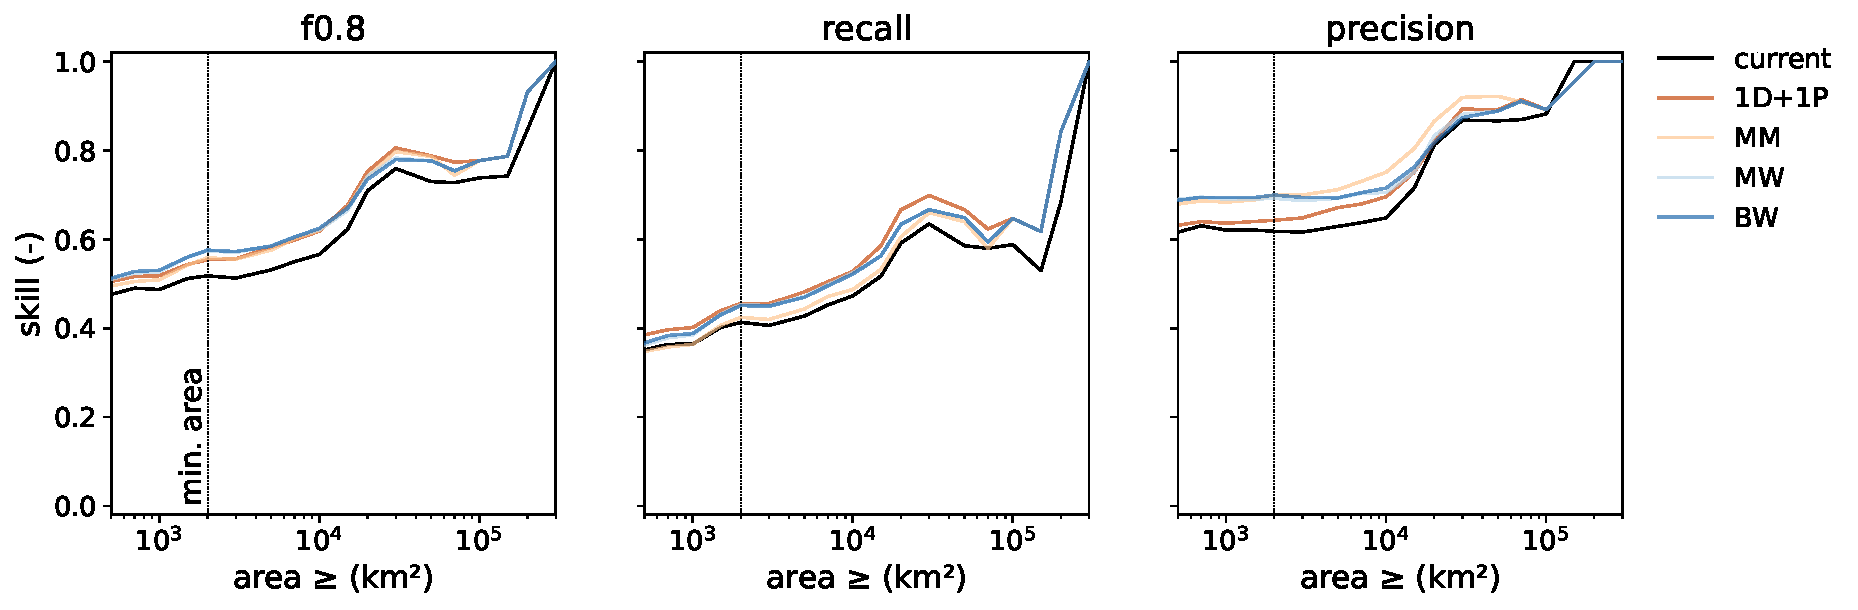
\includegraphics[width=1\linewidth]{figures/skill_vs_area_2000km2_1239points_060h.pdf}
    \caption{Evolution of skill with catchment area limit. Each plot represents a skill metric, with $f_{0.8}$ as the optimization target, and recall and precision as its components. In each of the plots, the black line represents the skill of the current notification criteria, while the colour lines depict the skill of the optimized criteria for the 4 combination methods. The vertical, dotted line indicates the catchment area limit currently applied in EFAS.}
    \label{fig:skill_area}
\end{figure}

The skill of the system improves with catchment area, as expected. For very large catchments, all three metrics reach their maximum value of 1. However, the skill curves do not increase continuously. Recall experiences a loss in skill for areas ranging from 30,000 to 70,000 km², leading to a decrease in $f_{0.8}$ values. This loss is caused by poor performance in the Guadiana, Seine, Loire, Rhone and Danube catchments. There is a notable gap between recall and precision, the components of the f-score, in both the optimized and current notification criteria, with precision consistently surpassing recall. 

The vertical line at 2000 km² illustrates the gain in skill achieved through optimization, which is sustained across all catchment area values. Reducing the catchment area limit results in minimal loss in $f_{0.8}$, suggesting that this criterion could be reduced without compromising skill. For instance, the Brier weighted approach at 1000 km² ($f_{0.8}=0.531$) exhibits slightly higher skill than the current criteria at 2000 km² ($f_{0.8}=0.518$). The relaxation of the catchment area limit impacts the f-score components differently. While precision remains unaffected, there is a loss in recall. To sum up, sending flood alerts to smaller catchments would marginally reduce the skill of the system, primarily due to an increase in missed events, without leading to more false alarm.

In the previous analysis, a fixed probability threshold was applied for all catchments, regardless of their area. We also investigated whether the skill of the system could be enhanced by adapting the probability threshold to the catchment area. Our rationale is rooted in the understanding that the level of uncertainty (model spread) in predictions differs between small and large catchments, suggesting that area-specific probability thresholds may enhance overall system skill. The results of this experiment are depicted in Figure \ref{fig:skill_area_probability}. Each plot represents a different combination method, comparing the f-score (solid lines) and the probability threshold (dashed lines) between the model optimized for a 2000 km² area limit (blue) and models optimized for increasing catchment area limits (orange). In order to compare the results of the two optimization runs, we kept a constant persistence value of 1/1, , which had been previously optimized for all combination methods within the lead time range of 2-5.5 days (refer to Table \ref{tab:COMB_optimization}).

\begin{figure}
    \centering
    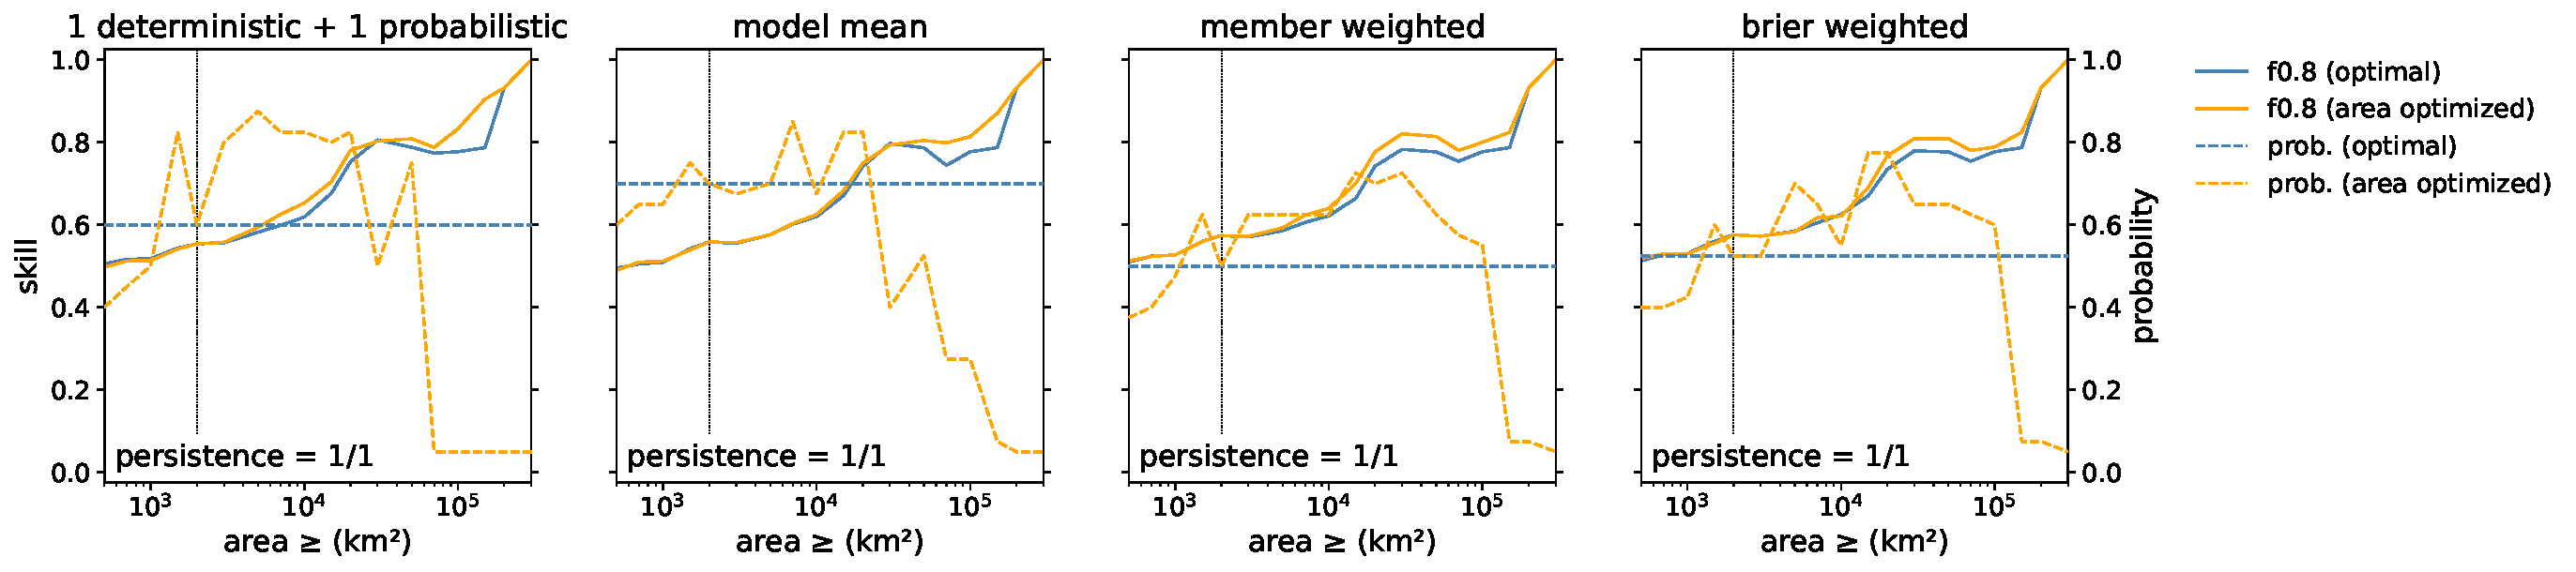
\includegraphics[width=1\textwidth]{figures/skill_vs_area_varying_probability_2000km2_1239points_060h.pdf}
    \caption{Comparison of the notification skill between a fixed (blue) and a area-specific (orange) probability threshold criterion for the lead time range from 2 to 5.5 days. Each plot depicts a different combination method, with solid lines representing the $f_{0.8}$ and dashed lines representing the probability threshold. The black, dotted, vertical line indicates the catchment area limit (2000 km²) used for optimizing the fixed probability threshold.}
    \label{fig:skill_area_probability}
\end{figure}

The skill measured as $f_{0.8}$ is very similar for both optimizations, especially for areas smaller than 2000 km². For larger areas, the main improvement is at the range between 30,000 and 100,000 km², for which the fixed criteria loses some skill. The evolution of the probability threshold with catchment area is somewhat erratic, likely due to uncertainty in defining the optimal value (refer to Figure \ref{fig:COMB_skill_probability}). Despite this, a general trend can discerned, with the threshold taking lower values for catchment areas smaller than 2000 km², peaking at approximately 100,000 km², and dropping to a minimum of 5\% for very large catchments. 

Overall, the experiment indicates that varying the probability threshold does not significantly improve the skill of the notification criteria. Therefore, for the sake of simplicity, a fixed probability threshold is recommended. 

\section{Discussion}
\label{sec:discussion}

Spatial and temporal framework

The definition of the spatial and temporal frame is often a limitation in studies that analyze the skill of ensemble flood forecasting systems \cite{Cloke2009}. Due to the rarity of flood events, the statistical robustness of such analysis relies on a limited and often highly correlated sample of events. To address this limitation, long-term and continental or global studies are advocated, such as the one presented here, which spans over a period of two and a half years and extends over a European domain. Nevertheless, our study would benefit from a larger sample of points and flood events. As shown in Figure \ref{fig:maps_BW}, there are many stations for which the skill metrics cannot be calculated due to null hits, misses or false alarms. A larger sample of observed events would reduce the susceptibility of the analysis to this issue. Two potential solutions emerge: extending the study period, which is limited by the availability of the HEPS forecasts (or reforecasts), or using a higher recurrence event threshold. We decided to work with a sample of stations, instead of all the river cells \cite{Bartholmes2009}, to limit the spatial correlation of events. Additionally, we tested removing stations with highly correlated discharge time series to further reduce correlation, but the results were similar and the sample of events much smaller, so we discarded that approach. 

In the optimization of the notification criteria, we set a catchment area limit of 2000 km², a threshold inherited from previous EFAS setups with lower spatial and temporal resolution. The results of this study (Figure \ref{fig:skill_area}) demonstrate that the current resolution of both NWP and hydrological models can produce skillful warnings at smaller catchments, which can significantly increase the number of stations and flood events analyzed, as shown in Figure \ref{fig:observed_vs_area}. In line with this, the new EFAS version 5 (\cite{EFASv5.0}) has increased spatial resolution from 5 km to 1 arc-minute, which is expected to further improve the skill of the system in smaller catchments. The skill of this new EFAS version will be analyzed as soon as a long enough period or reforecasts are available.

Selection of the target metric.

The selection of the target metric is a critical aspect in any skill analysis. \cite{Bartholmes2009} reviewed the desired characteristics of a skill score, and selected odds ratio, HK score and bias as their target metrics. In contrast, for our analysis, we selected the $f_{\beta}$ score, a metric commonly used in machine learning, but rarely applied in hydrology. The $f_{\beta}$ score has two interesting properties for analyzing a flood warning system. Firstly, it is based on the contingency table but avoids using true negatives, which could overestimate skill. Secondly, it allows for tailoring the notification criteria to the end user, as the $\beta$ parameter can be adjusted to penalize stronger misses or false alarms. For instance, Bouttier and Marchal \cite{Bouttier2023} used the $f_2$ score to optimize the probability threshold for high-intensity precipitation warnings in France. The $\beta$ value of 2 penalizes four times more missed events than false alarms, under the assumption that the cost of  being hit by an extreme event unprepared is larger than the cost of mobilising resources in a false alarm. In our study, we took the opposite approach and decided to minimize the number of false alarms by using a $\beta$ value of $0.8$. This decision was based on the fact that EFAS complements the national or regional systems by issuing medium-range flood warnings to the responsible administrations, not to the general public. The aim is to alert authorities only when there is substantial evidence that the event will occur, in order to avoid excessive notifications that could undermine their trust in the system. Additionally, the event threshold (5-year return period) corresponds to a recurrence time shorter that the flood protection levels in many European regions, so we assume that missing minor events will not be as costly as Bouttier and Marchal argue.

Comparison of deterministic and probabilistic NWP

The first objective of this study was to evaluate the skill of the different NWP within EFAS, with a specific focus on comparing deterministic and probabilistic models. Figure \ref{fig:BSS} demonstrates that probabilistic NWP outperforms deterministic NWP in terms of Brier skill score across all lead times, with the exception of short lead times where deterministic NWP approaches similar levels of skill. The picture is similar when applying the notification criteria and measuring warning skill in terms of $f_{0.8}$ (Figure \ref{fig:NWP_skill_leadtime} and Figure \ref{fig:NWP_skill_probability}). At their optimal notification criteria, the probabilistic NWPs, particularly ECMWF-ENS, outperform deterministic NWP. The skill of both types of NWP degrades with increasing lead time, casting doubt on their ability to issue flood alerts more than 5-6 days in advance. The effects of the probability threshold and persistence criteria differs depending on the nature of the NWP. The probability threshold has a substantial effect on the skill of probabilistic models, while it does not impact deterministic models due to their binary forecasted probabilities . Both COSMO-LEPS and ECMWF-ENS perform better at probability thresholds over 50\%, with a wide range of similarly performing values. On the contrary, persistence proves to be beneficial in improving the notification skill of deterministic NWPs, but it limits the skill of probabilistic models. Persistence, a.k.a. poor man's ensemble, is a method of creating an ensemble out of a deterministic forecast \cite{Cloke2009}. For instance, a persistence of 3/3 is an ensemble of 3 members with a probability threshold of 100\%. Our results show that while persistence removes the inherent erratic behaviour of deterministic models and notably improves their skill, it should not be applied to HEPS. 

Combination of NWP

The second objective of this study was to determine the appropriate method to combine several NWP models into a grand ensemble. Careful consideration is necessary in selecting this method to avoid diminishing the skill of the most proficient NWP within the grand ensemble. For instance, the current EFAS notification criteria limit the skill of the system to that of the highest-performing deterministic model (ECMWF-HRES), which is poorer than any of the individual probabilistic NWP (Figure \ref{fig:NWP_skill_probability}). This limitation is caused by a combination method (1D+1P) that assigns equal value to probabilistic and deterministic models, as well as the use of persistence. The challenge lies in finding a combination that enhances the skill of the best-performing NWP, which in the case of EFAS is the ECMWF-ENS.

Our findings demonstrate that ECWF-ENS is a very strong baseline, with only a few combination methods yielding marginal gains to its skill. The effectiveness of the grand ensemble is limited to the first 5 days lead time, when the total number of members is highest (73), particularly for lead times shorter than 2 days, when the deterministic models provide value. As an example, a simplistic approach like MM exhibits the highest skill within the shortest lead time range, potentially because it is the approach that assigns higher value to the deterministic models. Overall, the most promising approaches are the member-based (MW) and skill-based (BW) methods, as they outperform the baseline throughout the first 5 days lead time. Both methods have similar optimal notification criteria (no persistence and a probability threshold close to 50\%), and their success is based on granting most of the weight to ECMWF-ENS. However, the reason why they allocate this weight to ECMWF-ENS differs. In the case MW, it is coincidental that the most skillful model also possesses the largest number of members. On the contrary, BW grants greater value to ECMWF-ENS because it proved to be a superior model. If a more skillful model with fewer members would be added to the grand ensemble, BW would be able to extract that value, while MW would not. Therefore, we argue that skill-based combination methods are preferable. 

The decision of the most appropriate combination methods can not be based solely on skill metrics, but also consider other factors such as the  operational implementation effort, user comprehensibility, or the impact of adding or removing a NWP. Skill-based approaches, such as BW, are theoretically superior as the allocation of weights is based on quality rather than quantity. They are also the most robust when it comes to adding or removing NWP models. However, they are more challenging to implement and explain to end users. To derive the matrix of weights (Figure \ref{fig:weights}), a skill-based approach requires having an extensive period of reanalysis and reforecasts upfront, posing a substantial computational burden on system implementation. Additionally,  practitioners using the system forecasts would require additional training to understand that the ensemble members are not equiprobable, which would be easier to grasp, but there are some prevailing members.

There remains a question on the use of deterministic models in a grand ensemble dominated by a probabilistic NWP. When using a member-based combination, such as MW, deterministic models could be removed from the grand ensemble, as the weight allocated to them is so small that their inclusion barely affects the total probability. Skill-based approaches, instead, allocate larger weights to these models in the very first lead times, when they have proven value given their often higher resolution. The inclusion of deterministic models is a topic for future analysis, as the spatial resolution of deterministic and probabilistic NWP are nowadays similar, and centres such as the ECMWF plan to discontinue their deterministic models in favour of the ensembles.

\section{Conclusions}
\label{sec:conclusions}

This study describes a procedure to optimize warning thresholds for a hydrological ensemble prediction system (HEPS). We investigated the ability of deterministic and probabilistic Numerical Weather Prediction (NWP) models in providing correct flood warnings, and we explored the effects of the notification criteria, namely probability threshold and persistence. The final objective of the study is to device a method to combine several NWP into a grand ensemble in order to outperform the most proficient, individual NWP. Our study case is the European Flood Awareness System (EFASv4), a medium-range flood warning system.

The individual analysis of the NWPs demonstrated that probabilistic models, particularly ECMWF-ENS, provide better flood warnings than deterministic models, even for short lead times, where the latter show some skill. We discovered that the persistence criterion is useful to increase the skill of deterministic models, as it creates a pseudo-ensemble, but is counterproductive in the case of ensembles. The criterion that maximizes ensemble skill is the probability threshold, whose optimum shows a certain degree of uncertainty, but always exceeds a value of 50\%.

By default, the combination of several NWP into a grand ensemble does not improve the overall skill of the flood warning system. As an example, the current EFAS notification criteria, which uses four NWP, is outperformed by only using one NWP (ECWMF-ENS) with the adequate criteria. Two of the approaches tested in this work yield marginal gains in skill compared with the baseline in medium and short lead times. One of these approaches (named member weighted) assumes equiprobability among all the model runs, and the other one (named Brier weighted) assigns weights to each NWP at every lead time based on their Brier skill score. In our study case, these two approaches yield similar results because the most proficient NWP is also the one with the largest number of members. Despite that, we argue that the skill-based approach is conceptually more appropriate, gives significance to the inclusion of deterministic NWP in the ensemble, and would perform better if the set of NWP would change. However, other study cases may consider other factors such implementation costs or explainability in the selection of the combination method.

Finally, we explored how catchment area affects the notification skill, with the idea of relaxing the current notification criterion that establishes a minimum catchment area. The results indicate that skill deteriorates with decreasing catchment area, as other studies report, but the improvements in meteorological and hydrological models over the last decade allow for a reduction in the minimum catchment area. We have proven that with the optimized criteria we can halve the area limit, therefore cover a larger area, and achieve a similar performance as in the current system setup. We expect that the skill at smaller catchments will be positively affected by the release of the new EFAS version with a higher spatial resolution.


--- 
the skill of the flood warnings compared the skill of the flood warnings based on individual numerical weather prediction (NWP) models, both deterministic and probabilistic, and we examined different methods of combining the NWP into a grand ensemble with the purpose of improving the overall skill of the system. Our study case is the European Flood Awareness System (EFASv4), a medium-range flood warning system.

This study has analysed the skill of the notification criteria based on EFAS4 discharge simulations. The benchmark done with the current operational criteria shows that the system has an overall medium skill, with a tendency to underpredict events, i.e., to produce more missed events than false alarms.

An analysis of the individual meteorological models has shown that the two probabilistic models (COSMO-LEPS and ECMWF-ENS) individually outperform the current criteria, which uses four models. ECMWF-ENS is the most skillful model and will be used as a baseline for the optimization of the combination methods. The optimization of the notification criteria for the individual models NWP indicates that persistence is only a useful criteria for deterministic models, and that there is a certain degree of uncertainty in the definition of the optimal probability threshold for the probabilistic models (a wide range of probabilities perform equally good).

A second analysis compared the best NWP model against four different methods of combining the NWP models. From more simple to more complex, the model mean assigns the same value to all 4 NWP models, the member weighted method assigns equal value to every model run (probabilistic models prevail over deterministic), and the Brier weighted method uses the Brier score derived in the first analysis to weight the models according to their skill. The results prove that ECMWF-ENS is a baseline difficult to beat. Two approaches stand out as the most appropriate: member weighted  and Brier weighted . When looking at the most representative lead time range (60-132 h), they both outperform slightly the baseline, which means that they are able to add value from COSMO-LEPS, DWD or ECMWF-HRES to it. Both approaches optimized similar criteria: no persistence and a probability threshold around 50\%. The selection of one of these two approaches must be based on implementation issues, ability to add/remove meteorological forcing, and the interpretability on the part of EFAS partners.

Finally, we have analysed the possibility of relaxing the current criterion that establishes a minimum catchment area of 2,000 km². The results indicate that skill deteriorates with decreasing catchment area at a rather small rate. We have proven that with the optimized criteria we can achieve a similar performance at 1,000 km² as that of the current criteria at 2,000 km². 

Future work:

\begin{itemize}
\item In the future, when EFAS5 reforecast will be available, it will be interesting to redo the analysis for this version, especially regarding the question about reducing the area threshold.
\end{itemize}

\section{Data availability}

The reanalysis and forecast discharge data is available at the \href{https://cds.climate.copernicus.eu}{Climate Data Store of the Copernicus Climate Change Service}. All the scripts, pre-processed data and results of the study can be found in this \href{https://github.com/casadoj/EFAS_skill}{GitHub repository}.

%% The Appendices part is started with the command \appendix;
%% appendix sections are then done as normal sections
\appendix

\section{Sample Appendix Section}
\label{sec:sample:appendix}
Lorem ipsum dolor sit amet, consectetur adipiscing elit, sed do eiusmod tempor section...

%% If you have bibdatabase file and want bibtex to generate the
%% bibitems, please use
%%
\bibliographystyle{elsarticle-harv} 
\bibliography{EFAS_skill}

%% else use the following coding to input the bibitems directly in the
%% TeX file.

% \begin{thebibliography}{00}

% %% \bibitem[Author(year)]{label}
% %% Text of bibliographic item

% \bibitem[ ()]{}

% \end{thebibliography}
\end{document}

\endinput
%%
%% End of file `elsarticle-template-harv.tex'.
